%-------------------------------------------------------%
%      HPCCF Virt. Workshop Presentation CM             %
%-------------------------------------------------------%
\documentclass[english,xcolor=pdftex,dvipsnames,compress,aspectratio=169]{beamer}


%\setbeamertemplate{mini frames}[box]
\usepackage{babel}
\usepackage[utf8]{inputenc}
\usepackage[T1]{fontenc}
\usepackage{amsfonts,amsmath,amssymb}
\usepackage{wrapfig}
\usepackage{pifont}

\usepackage{color,colortbl}
\usepackage{upquote}
\usepackage{tcolorbox}
% \usepackage{showexpl}
% \lstset{
%     basicstyle=\ttfamily\small,
%     commentstyle=\itshape\ttfamily\small,
%     showspaces=false,
%     showstringspaces=false,
%     breaklines=true,
%     breakautoindent=false,
%     captionpos=t
% }

\definecolor{pblue}{RGB}{45,106,148}
\definecolor{pdarkblue}{RGB}{35,71,100}
\definecolor{plightblue}{RGB}{90,159,212}
\definecolor{pyellow}{RGB}{255,212,59}
\definecolor{pdarkyellow}{RGB}{255,188,41}
\definecolor{orange}{RGB}{255,165,0}
\definecolor{plightyellow}{RGB}{255,232,115}
\definecolor{pdarkgrey}{RGB}{100,100,100}
\definecolor{pgrey}{RGB}{153,153,153}
\definecolor{plightgrey}{RGB}{233,233,233}
\definecolor{plightgrey2}{RGB}{247,247,247}
\definecolor{pnavy}{RGB}{0,0,170}
\definecolor{BrickRed}{RGB}{150,22,11}
\definecolor{BlueViolet}{RGB}{138, 43, 226}
\definecolor{PineGreen}{RGB}{0, 51, 0}
\definecolor{light-gray}{gray}{0.95}

\definecolor{UniRot}{RGB}{193,0,42}
\definecolor{UniDunkelGrau}{RGB}{99,99,99}
\definecolor{UniHellGrau}{RGB}{172,172,172}

\definecolor{UrlColor}{rgb}{0,0.08,0.45}
\definecolor{links}{rgb}{0,0,0}

\usetheme{Goettingen_MZ_twist} % Pittsburgh, CambridgeUS
%\usecolortheme{beaver} %wolverine | crane | beaver | seahorse
%\useinnertheme{rounded} 
%\useoutertheme{default}
\usefonttheme{default}
%\setbeamercovered{transparent}
\setbeamertemplate{footline}[frame number]
\setbeamersize{text margin left=0.5cm, text margin right=0.5cm}

% \setbeamercolor{structure}{fg=UniRot}% to modify  immediately all palettes
% \setbeamercolor{title}{fg=UniRot}
% \setbeamercolor{title in head/foot}{fg=UniRot}
% 
% \setbeamercolor{block title}{bg=UniRot!20,fg=darkred}
% \setbeamercolor{block body}{fg=black, bg=plightgrey2}
% 
% % \setbeamercolor{block title}{fg=white,bg=orange}
% \setbeamercolor{block title alerted}{fg=white,bg=UniRot}
% \setbeamercolor{block title example}{fg=white,bg=PineGreen!80}

\graphicspath{{../2019-06-isc/}{../2019-06-isc/fig/}{img/}{../logo/}{images/}}

\usepackage{tikz}
\usetikzlibrary{arrows,shapes,backgrounds,positioning,shadows,decorations,trees,decorations.pathreplacing}


\addtobeamertemplate{footline}{}{%
\begin{tikzpicture}[remember picture,overlay]
\node[anchor=south west,yshift=2pt] at (current page.south west) {
\includegraphics[height=0.8cm]{./images/logo_schriftzug.jpg}};
\end{tikzpicture}}



\title{\Large HPCCF Taking the Exam}
\author{Christian Meesters (+ HPC Certification Forum)}
\date{2021-06-29}
%\authorURL{https://hpc-certification.org}
%\authorFooter{Christian Meesters \& Julian Kunkel}
%\venue{HPCCF Virtual Workshop}
\institute{HPC Group -- Johannes Gutenberg-University of Mainz}
%\groupLogo{
\includegraphics[width=2.5cm]{hpccf-small}}

\usepackage{multicol}

\usepackage{hhline}

\usepackage{times}

% will decrease the font size for one frame
\newcommand\Fontvi{\fontsize{6}{7.2}\selectfont}

\usepackage{verbatim}
\usepackage{listings}

\lstloadlanguages{Python,bash,C++}
\lstset{showspaces=false,
basicstyle=\small,
showstringspaces=false}


%default python listings:
\lstdefinestyle{Python}
{
  language=Python,
  basicstyle=\small,
  showstringspaces=false,
  stepnumber=5,
  numberstyle=\tiny,
  numbersep=5pt,
  showspaces=false,
  frame=single,
  framerule=0.4pt,
  rulecolor=\color{pgrey},
  backgroundcolor=\color{white},
  stringstyle=\color{BrickRed},
  keywordstyle=\color{BlueViolet}\bfseries,
  commentstyle=\color{PineGreen}\bfseries,
  identifierstyle={},
  emph={[10]self}, emphstyle={[10]\color{pblue}},
  emph={[11]yield}, emphstyle={[11]\color{pblue}},
}

%default python listings:
\lstdefinestyle{C++}
{
  language=C++,
  basicstyle=\small,
  showstringspaces=false,
  stepnumber=5,
  numberstyle=\tiny,
  numbersep=5pt,
  showspaces=false,
  frame=single,
  framerule=0.4pt,
  rulecolor=\color{pgrey},
  backgroundcolor=\color{white},
  stringstyle=\color{BrickRed},
  keywordstyle=\color{BlueViolet}\bfseries,
  commentstyle=\color{PineGreen}\bfseries,
  identifierstyle={},
  emph={[10]self}, emphstyle={[10]\color{pblue}},
  emph={[11]yield}, emphstyle={[11]\color{pblue}},
}

\newcommand{\CC}{C\nolinebreak\hspace{-.05em}\raisebox{1ex}{\tiny\bf +}\nolinebreak\hspace{-.10em}\raisebox{1ex}{\tiny\bf +}}

%default shell listings:
\lstdefinestyle{Shell}
{
  language=Bash,
  basicstyle=\ttfamily\small,
  showstringspaces=false,
  frame=single,
  framerule=0.4pt,
  rulecolor=\color{pgrey},
  backgroundcolor=\color{plightgrey2},
  stringstyle=\color{BrickRed},
  keywordstyle=\color{BlueViolet},
  commentstyle=\color{PineGreen}\bfseries,
  identifierstyle=\color{black},
  emph={[10]\$,>>>}, emphstyle={[10]\color{pblue}},
  moredelim=**[is][\bfseries\color{red}]{@}{@}
}

%default plain listings (e.g. for config files):
\lstdefinestyle{Plain}
{ 
  stepnumber=5,
  numberstyle=\tiny,
  numbersep=5pt,
  language=Bash,
  basicstyle=\ttfamily\small,
  showstringspaces=false,
  frame=single,
  framerule=0.4pt,
  rulecolor=\color{pgrey},
  backgroundcolor=\color{plightgrey2},
  stringstyle=\color{black},
  keywordstyle=\color{black},
  commentstyle=\color{blue}\bfseries,
  identifierstyle=\color{black},
  emph={[10]\$,>>>}, emphstyle={[10]\color{pblue}}
}
\lstdefinelanguage{XML}
{
  frame=single,
  framerule=0.4pt,
  rulecolor=\color{pgrey},
  backgroundcolor=\color{plightgrey2},
  stringstyle=\color{black},
  keywordstyle=\color{black},
  commentstyle=\color{blue}\bfseries,
  identifierstyle=\color{black},
  emph={[10]\$,>>>}, emphstyle={[10]\color{pblue}}
  morestring=[b]",
  morestring=[s]{>}{<},
  morecomment=[s]{<?}{?>},
  morekeywords={xmlns,version,type}% list your attributes here
}

\newcommand{\bibtex}{\textsc{Bib}\TeX}

%%% https://tex.stackexchange.com/questions/99316/symbol-for-external-links
\newcommand{\LinkSymbol}{%
  \tikz[x=1.2ex, y=1.2ex, baseline=-0.05ex]{% 
    \begin{scope}[x=1ex, y=1ex]
      \clip (-0.1,-0.1) 
      --++ (-0, 1.2) 
      --++ (0.6, 0) 
      --++ (0, -0.6) 
      --++ (0.6, 0) 
      --++ (0, -1);
      \path[draw, 
      line width = 0.5, 
      rounded corners=0.5] 
      (0,0) rectangle (1,1);
    \end{scope}
    \path[draw, line width = 0.5] (0.5, 0.5) 
    -- (1, 1);
    \path[draw, line width = 0.5] (0.6, 1) 
    -- (1, 1) -- (1, 0.6);
  }
}
\newcommand{\lhref}[2]{\href{#1}{#2\,\LinkSymbol}}

%%%% shortcuts for uniform appearance of common strings %%%%
\newcommand{\slurm}{\textsc{slurm}~}
\makeatletter
\newcommand{\rmnum}[1]{\romannumeral #1}
\newcommand{\Rmnum}[1]{\expandafter\@slowromancap\romannumeral #1@}
\makeatother
\usepackage{xspace}
\newcommand{\mogon}{\textsc{mogon}\xspace}
\newcommand{\mogonI}{\textsc{mogon}\,\Rmnum{1}\xspace}
\newcommand{\mogonII}{\textsc{mogon}\,\Rmnum{2}\xspace}

\setcounter{tocdepth}{1}


\venue{Parallel event to ISC HPC}
\institute{HPC Group Mainz, Germany}
\groupLogo{
\includegraphics[width=2.5cm]{hpccf-small}}
\titleLogo{ 
\includegraphics[height=2.8cm]{blur-book-stack-books-590493}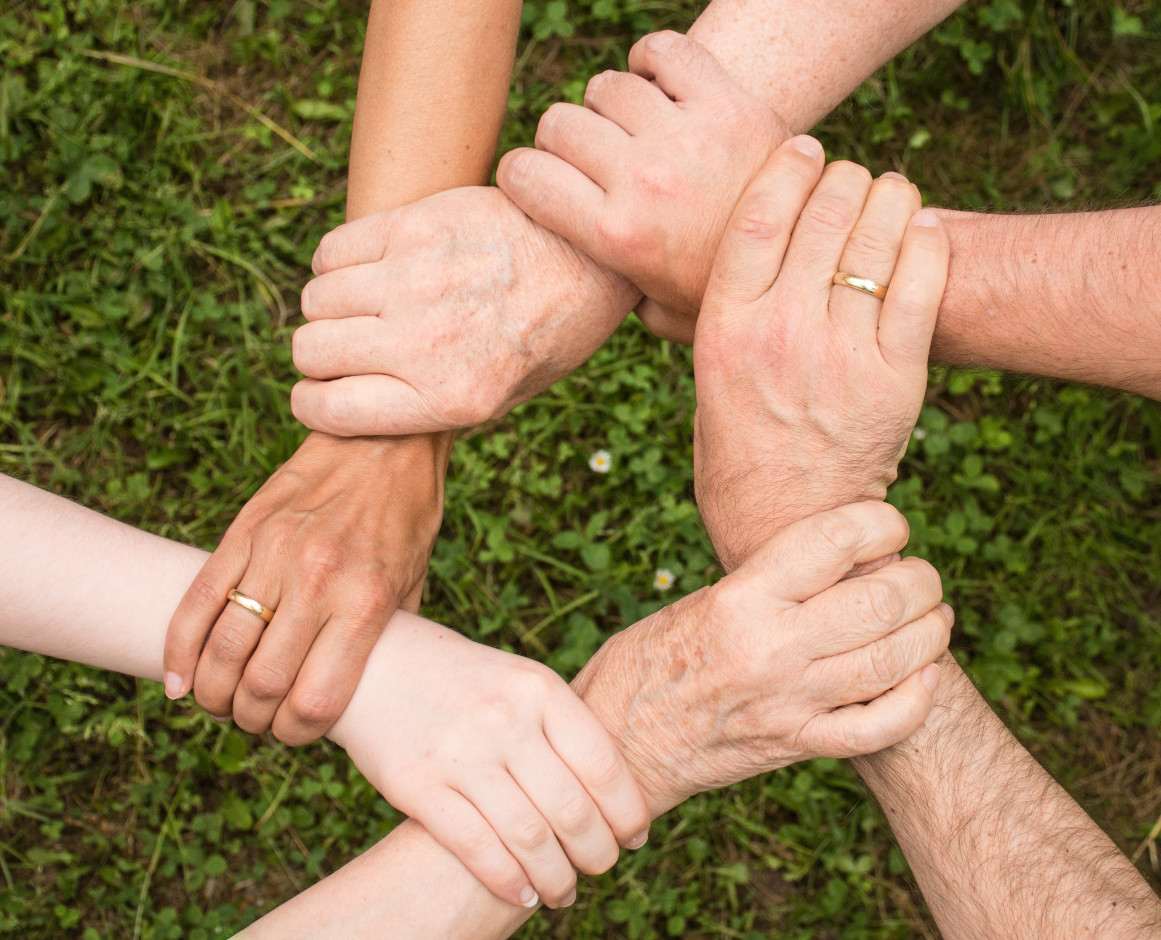
\includegraphics[height=2.8cm]{ground-group-growth-461049}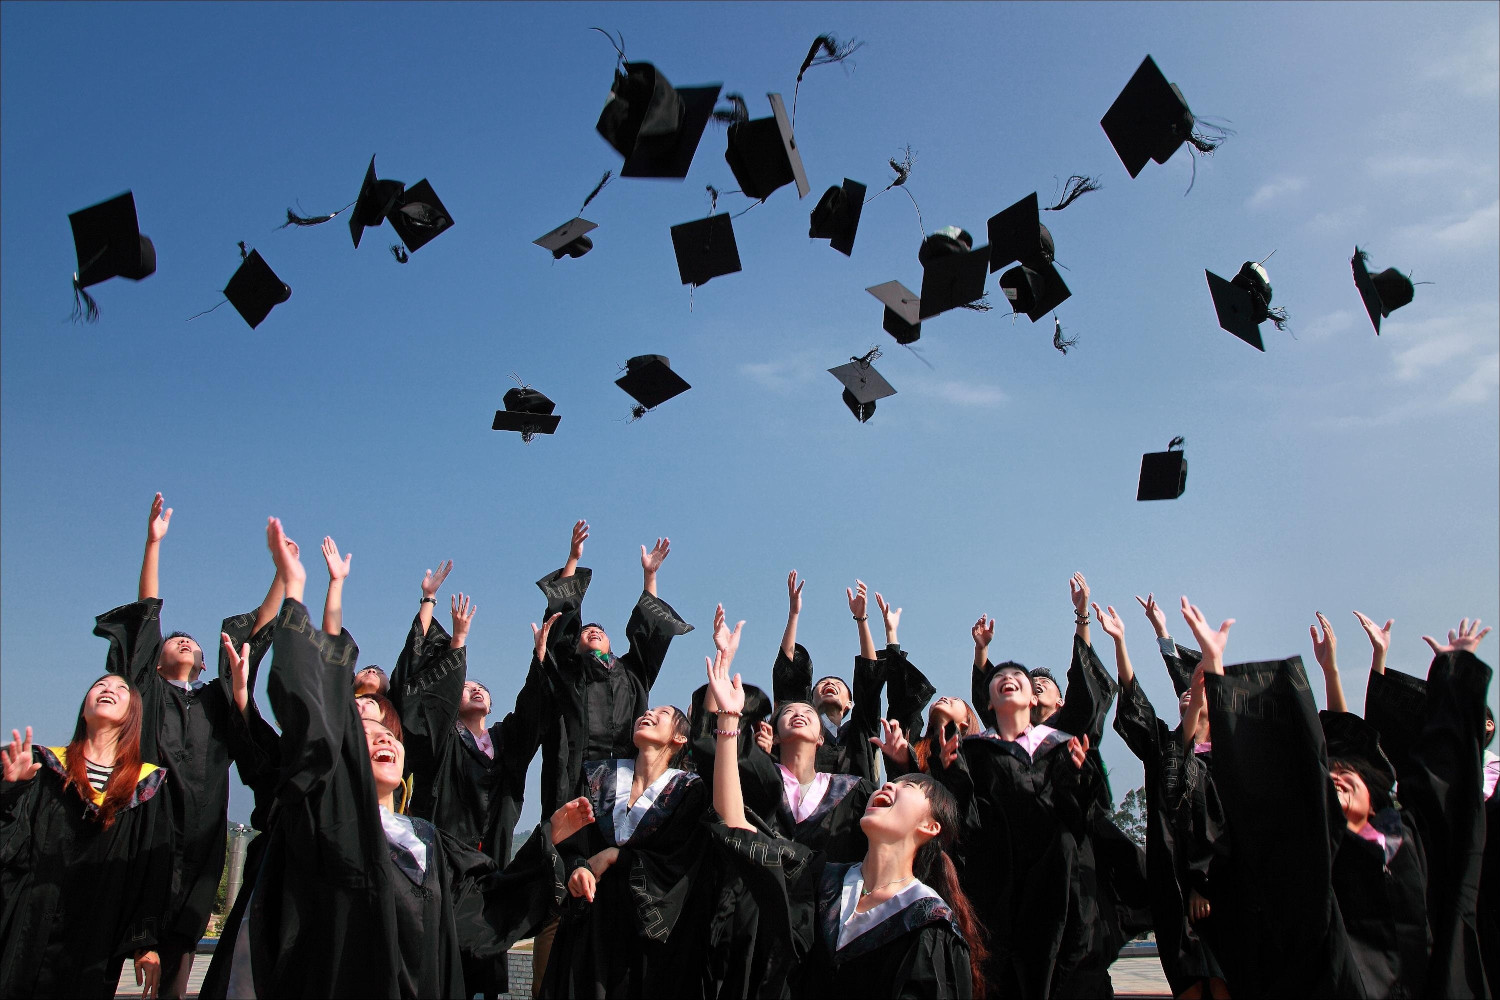
\includegraphics[height=2.8cm]{accomplishment-ceremony-college-267885}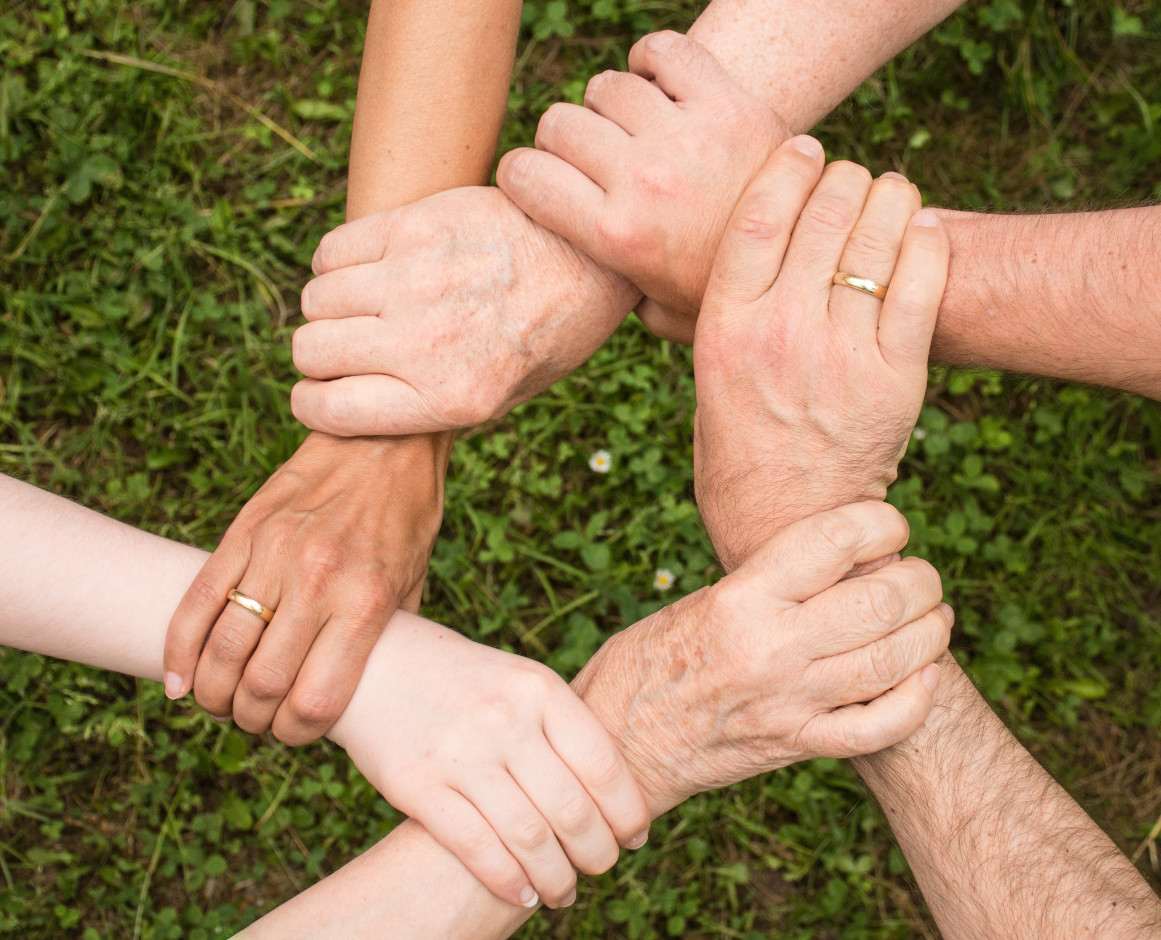
\includegraphics[height=2.8cm]{ground-group-growth-461049}
\includegraphics[height=2.8cm]{blur-book-stack-books-2}}


%%%%%%%%%%%%%%%%%%%%%%%%%%%%%%%%%%%%%%%%%%%%%%%%%%%%%%%%%%%%%%%%%%%%%%%%%%%%%%%%
%%%%%%%%%%%%%%%%%%%%%%%%%%%%%%%%%%%%%%%%%%%%%%%%%%%%%%%%%%%%%%%%%%%%%%%%%%%%%%%%
\begin{document}
%%%%%%%%%%%%%%%%%%%%%%%%%%%%%%%%%%%%%%%%%%%%%%%%%%%%%%%%%%%%%%%%%%%%%%%%%%%%%%%%
%%%%%%%%%%%%%%%%%%%%%%%%%%%%%%%%%%%%%%%%%%%%%%%%%%%%%%%%%%%%%%%%%%%%%%%%%%%%%%%%

% Passe captions an
\setbeamertemplate{caption}{\insertcaption}
% \setbeamerfont{caption}{size=\scriptsize}
\setlength\abovecaptionskip{-2.5pt}
\setlength\belowcaptionskip{0pt}



% For every picture that defines or uses external nodes, you'll have to
% apply the 'remember picture' style. To avoid some typing, we'll apply
% the style to all pictures.
\tikzstyle{every picture}+=[remember picture]
\tikzstyle{na} = [baseline=-.5ex]

%%%%%%%%%%%%%%%%%%%%%%%%%%%%%%%%%%%%%%%%%%%%%%%%%%%%%%%%%%%%%%%%%%%%%%%%%%%%%%%% 
\begin{frame}[plain]{}
  \maketitle
\end{frame}

%%%%%%%%%%%%%%%%%%%%%%%%%%%%%%%%%%%%%%%%%%%%%%%%%%%%%%%%%%%%%%%%%%%%%%%%%%%%%%%% 
% \begin{frame}
%     \frametitle{Outline}
%     \tableofcontents
% \end{frame}

\section[For- and Background]{For- and Background}



\subsection{Certification Process}

\begin{frame}
  \frametitle{Getting Started}
  \begin{columns}
    \begin{column}{.5\textwidth}
       \centering
      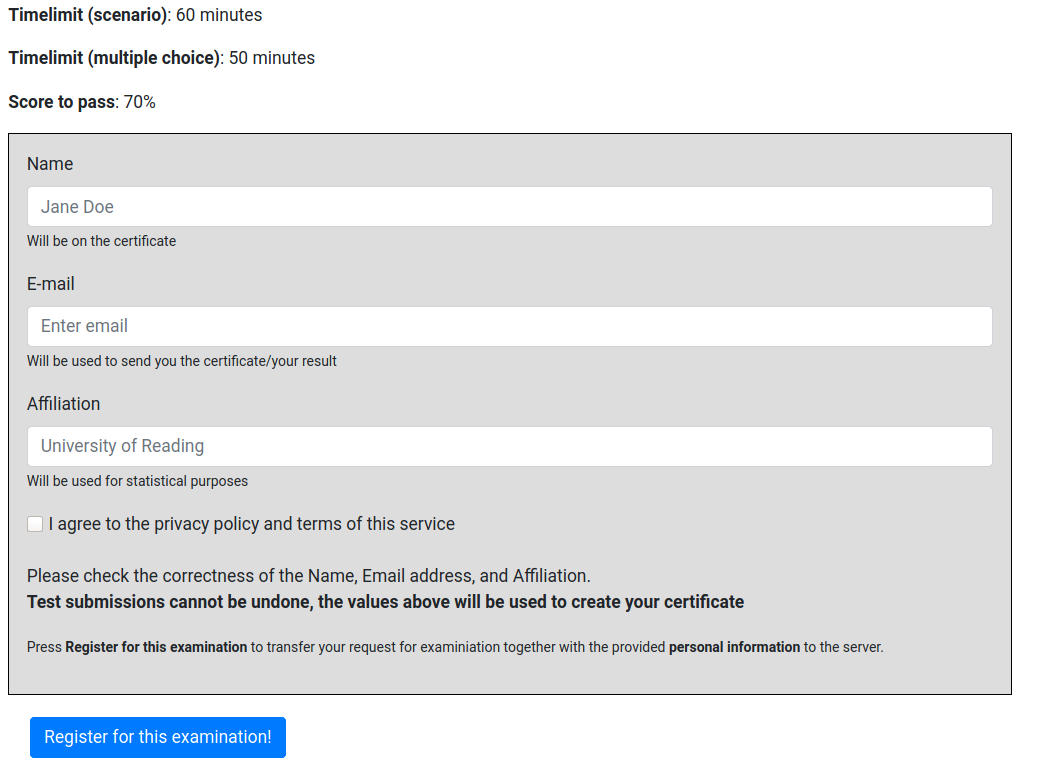
\includegraphics[width=0.9\textwidth]{images/getting_started}
    \end{column}
    \begin{column}{.5\textwidth}
      \begin{itemize}[<+->]
       \item navigate to the web page
       \item select the appropriate skill to be tested for
       \item submit Name \& Affiliation (which are needed for the certificate) \& and email
      \end{itemize}
      \pause
      $\curvearrowright$ a mail will be send containing links and keys for the actual exam (valid for 24 h)
    \end{column}
  \end{columns}
  
\end{frame}

\begin{frame}
 \frametitle{Background: Selecting the Questions}
 \begin{columns}
    \begin{column}{.5\textwidth}
       \centering
      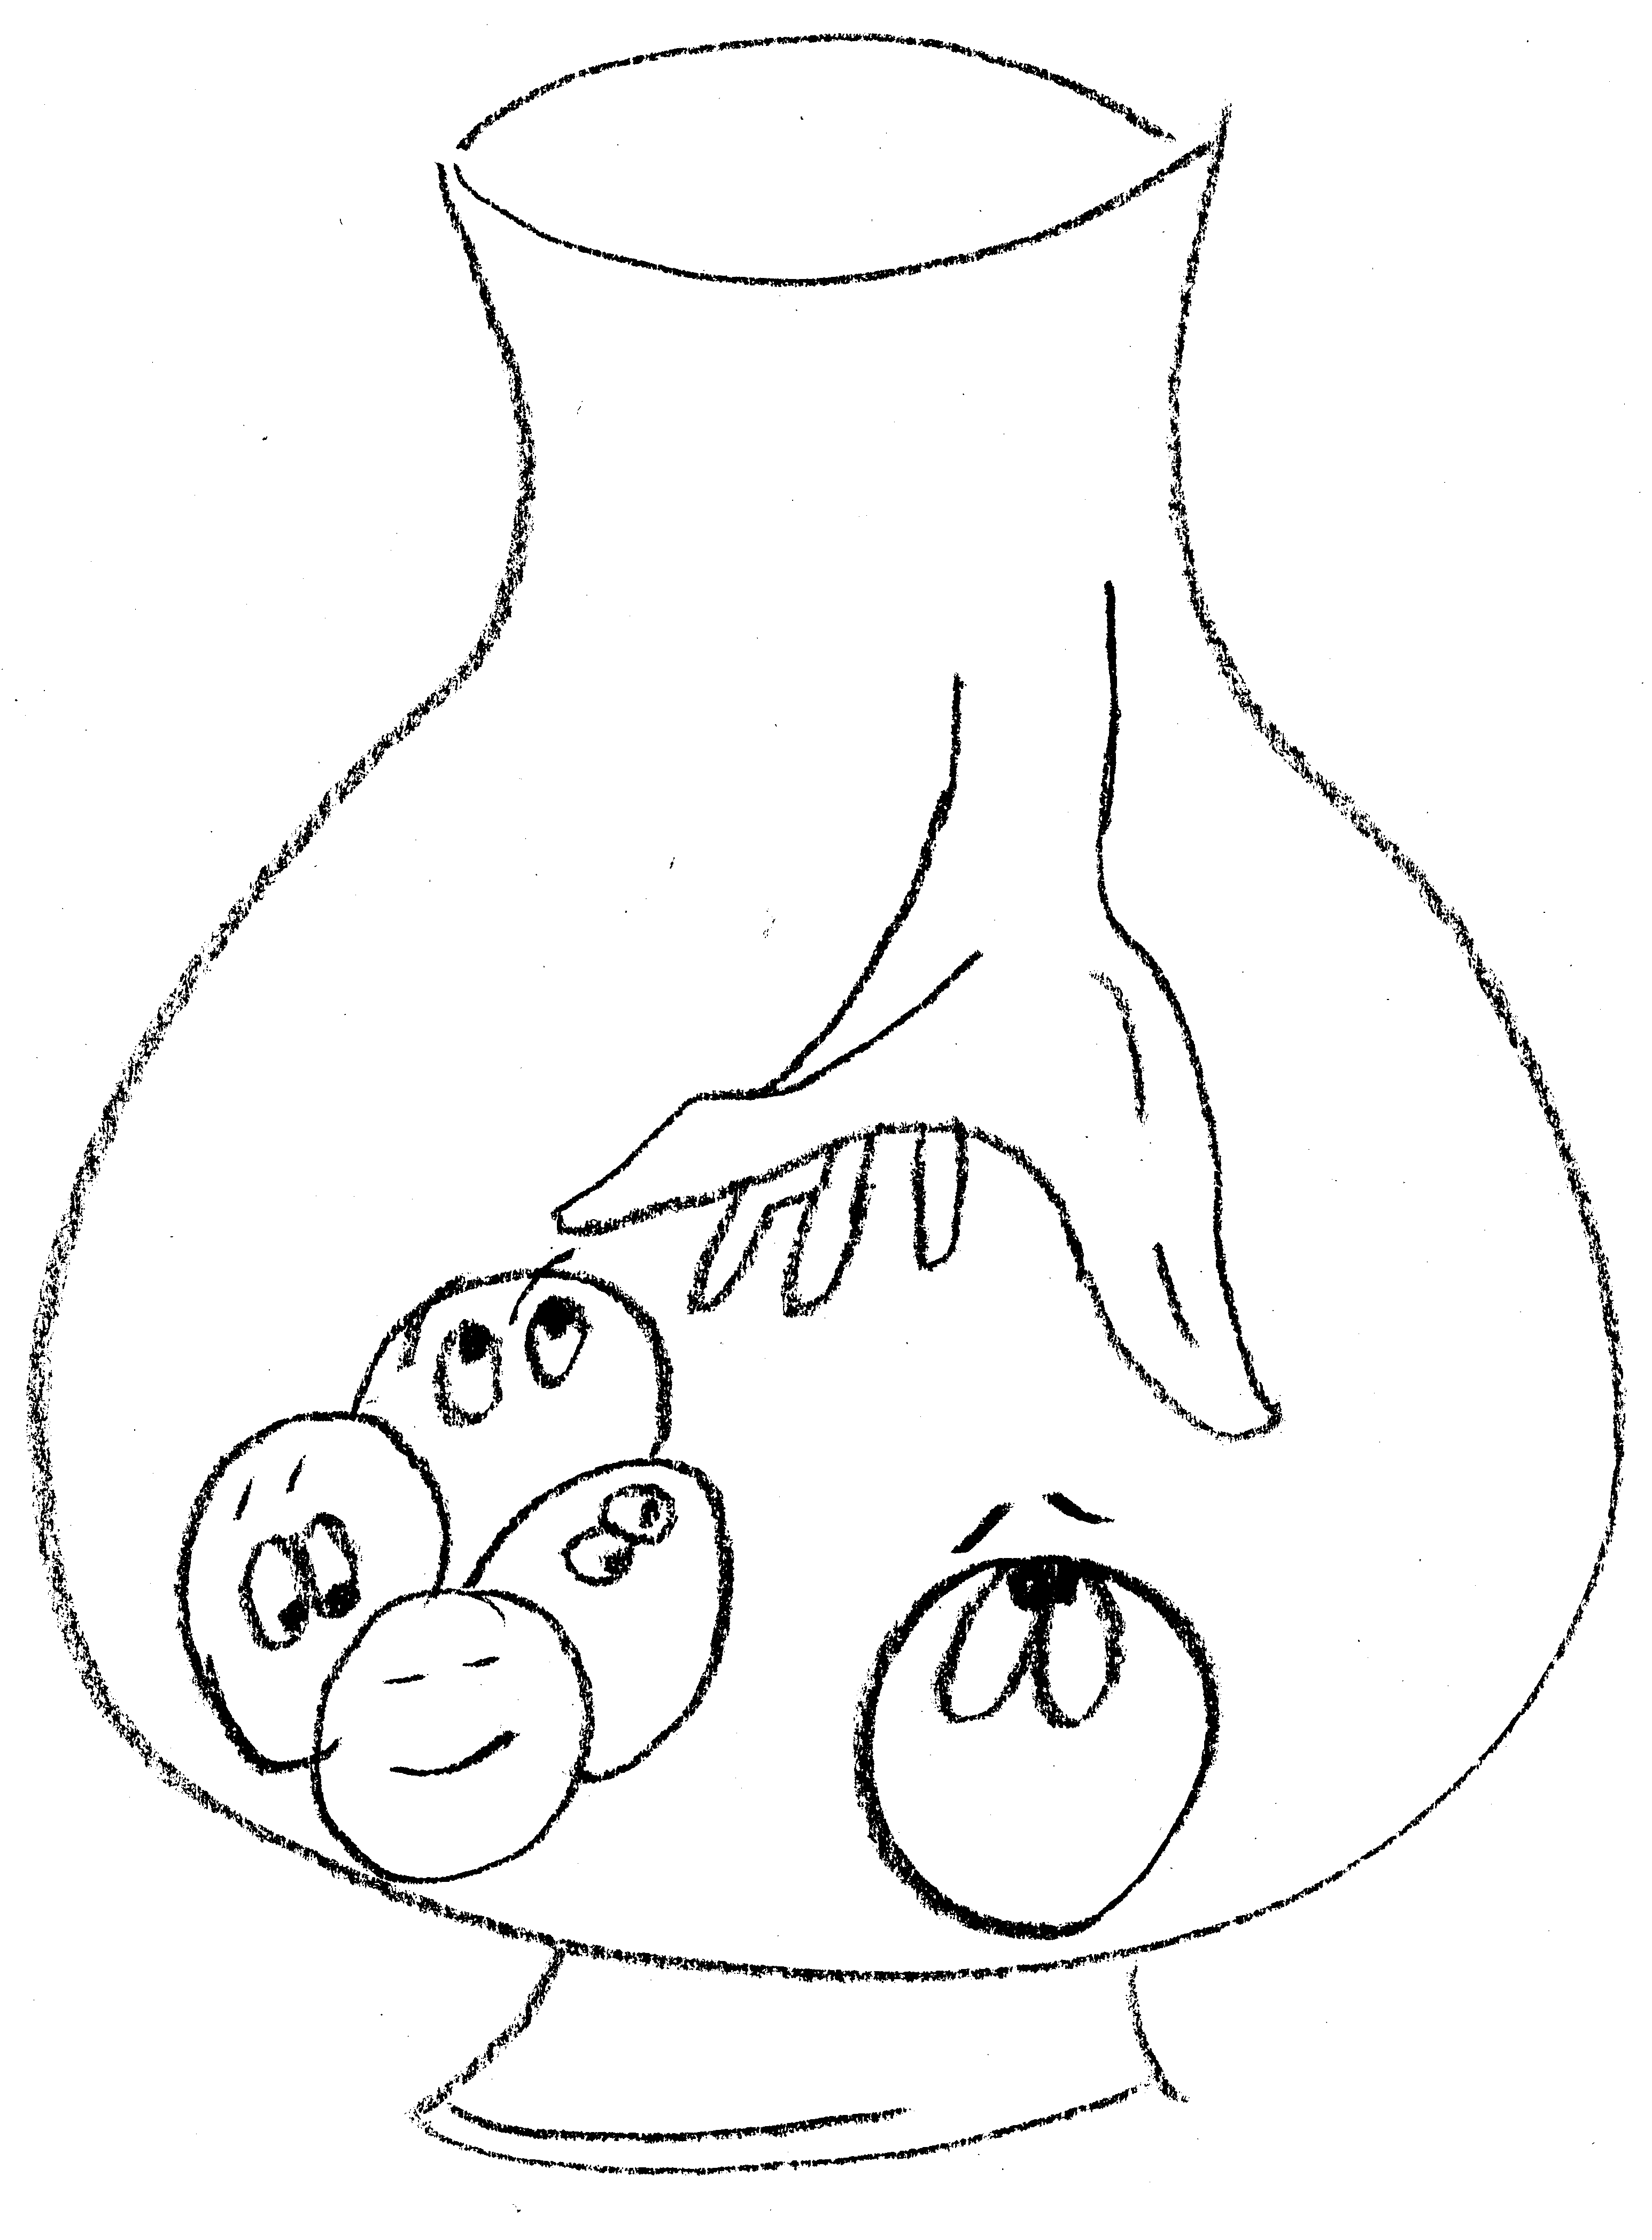
\includegraphics[width=0.6\textwidth]{images/urn}
    \end{column}
    \begin{column}{.5\textwidth}
      Questions are randomly choosen from a pool:
         the pool may itself be a bundle of sub-branches of the skill tree
              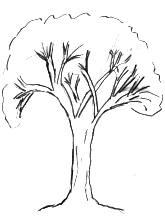
\includegraphics[width=0.1\textwidth]{images/tree_tiny}
        
      $\curvearrowright$ All examinations will be based on different sets of questions.
    \end{column}
  \end{columns}
\end{frame}

\begin{frame}
  \frametitle{On Cheating}
  \begin{columns}
   \begin{column}{.5\textwidth}
     \begin{enumerate}
      \item By confronting with random questions no perfect preperation can be accomplished.
      \item There is a time-limit per question.
      \item A registration prior to a test session is required.
     \end{enumerate}
    No online system without ID checks and other measures is safe against cheating! Yet, our measures will raise awareness.
   \end{column}
   \begin{column}{.5\textwidth}
       \centering
      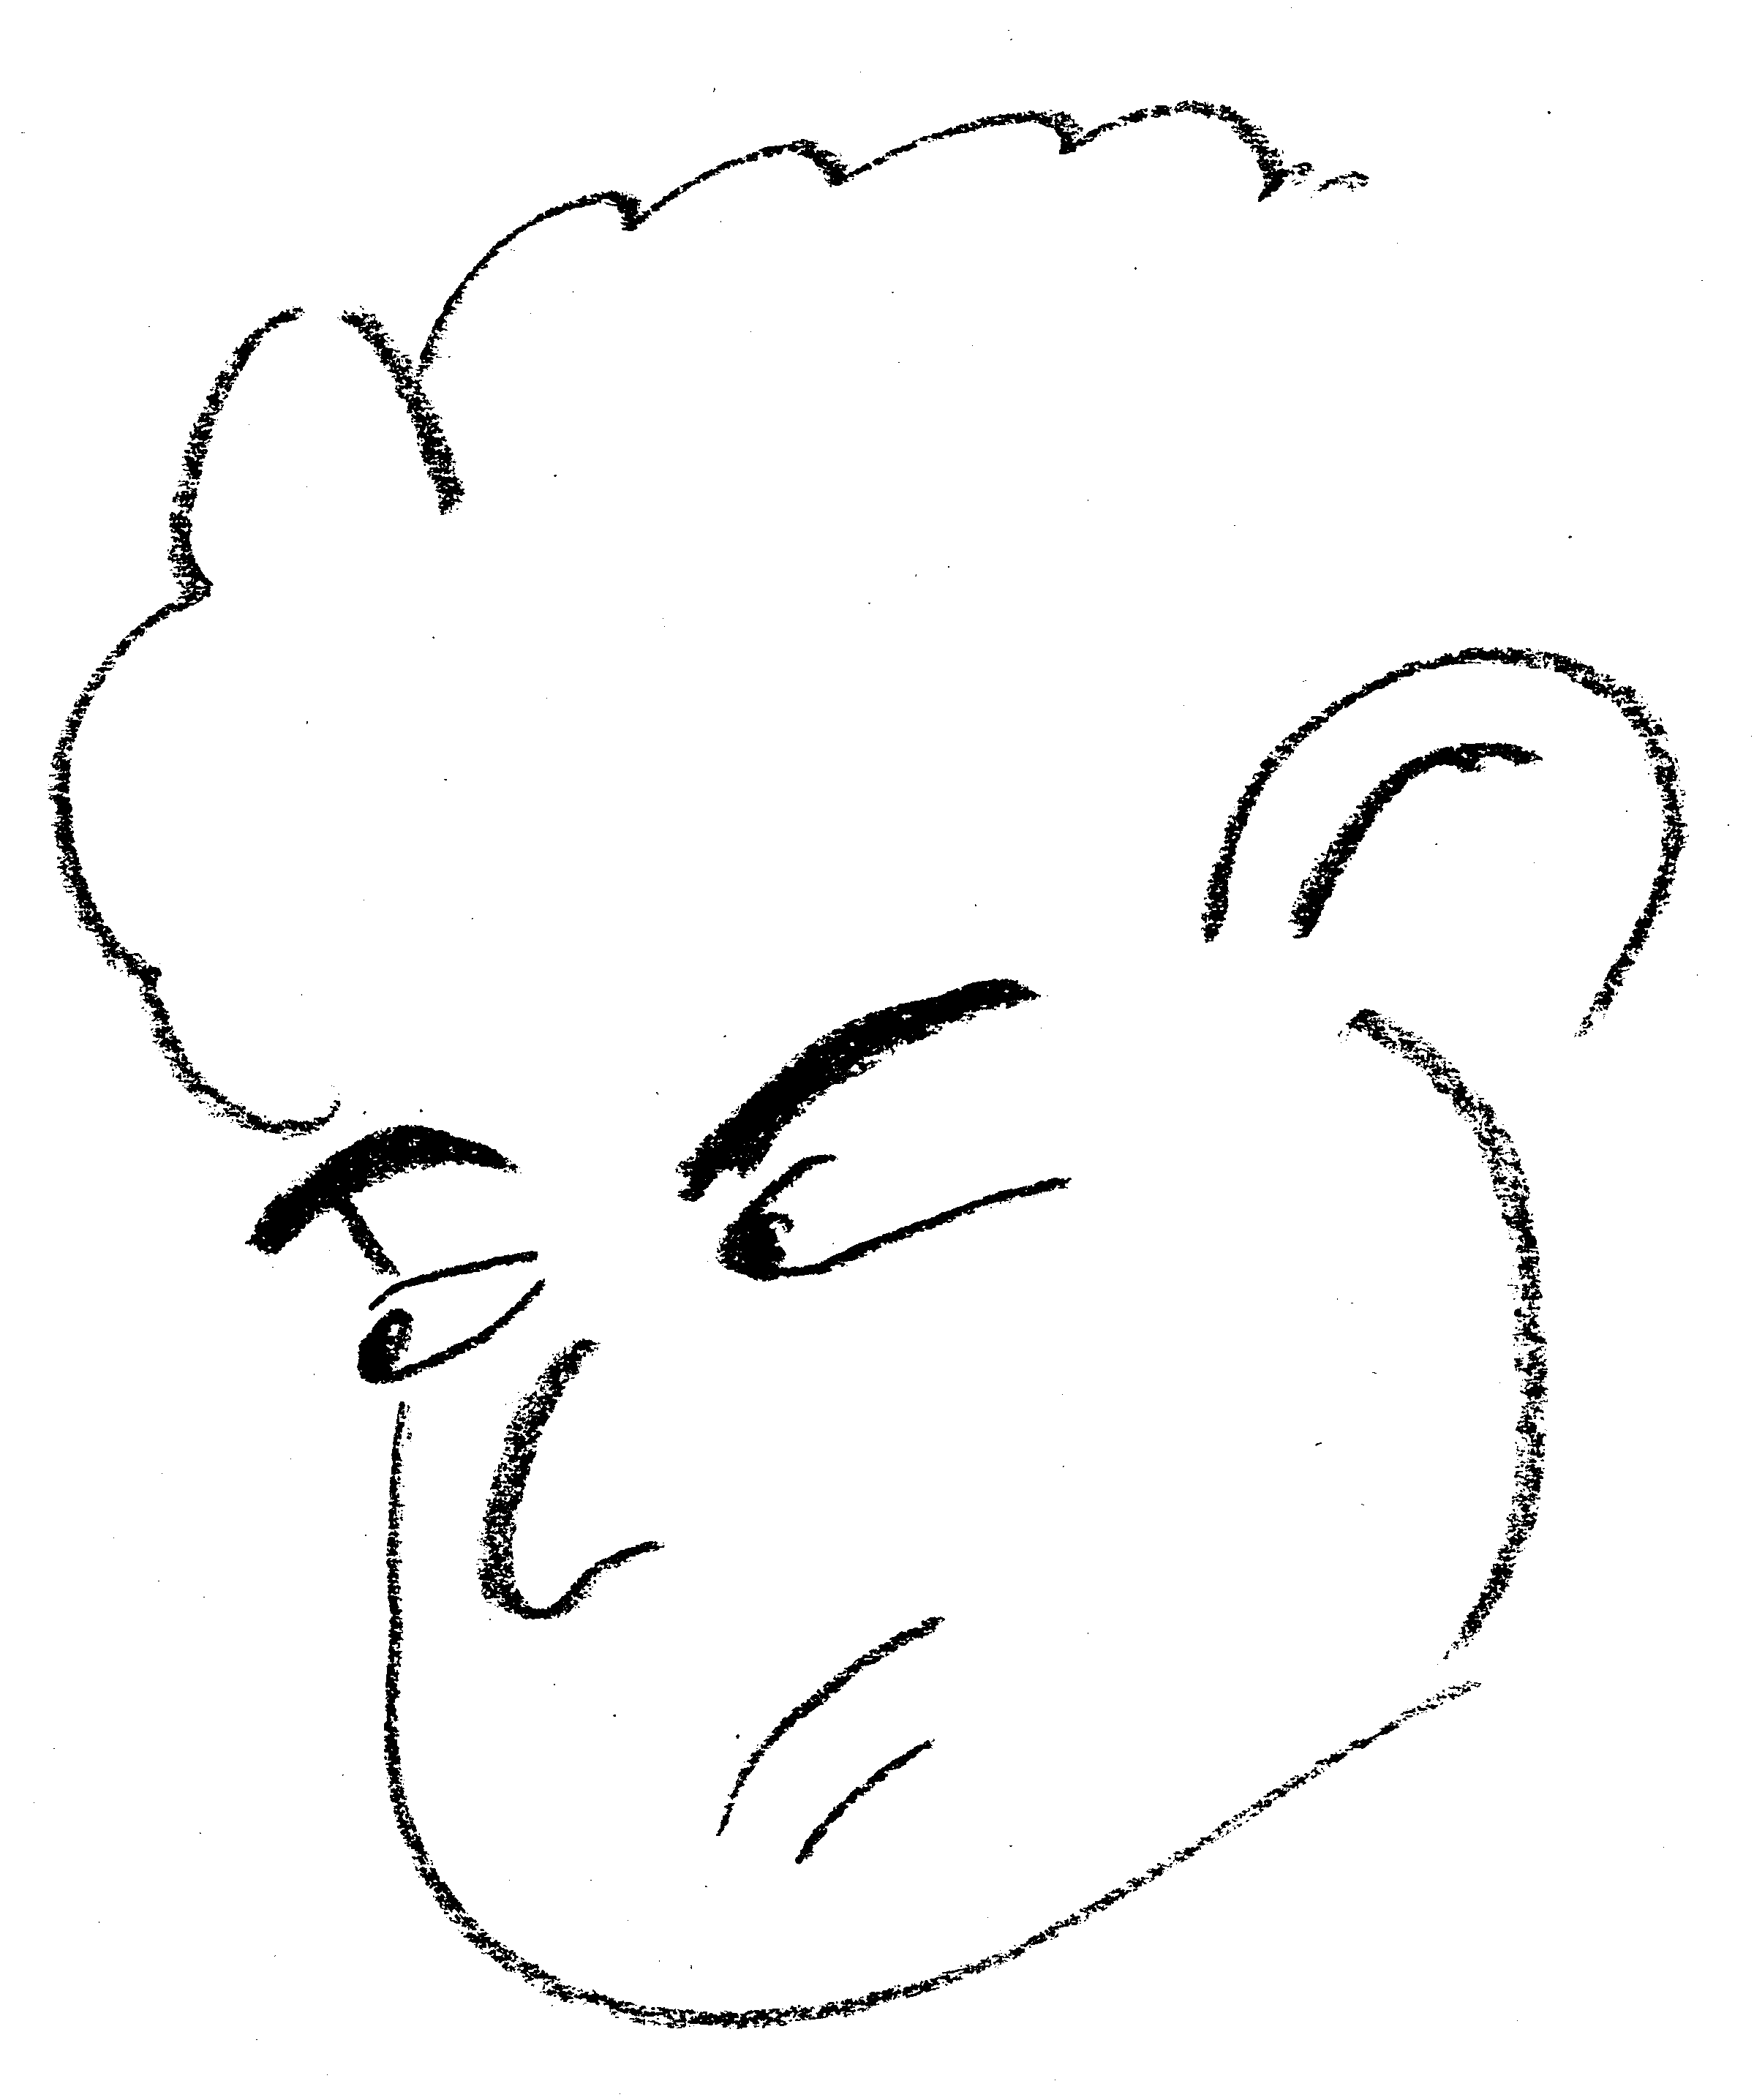
\includegraphics[width=0.6\textwidth]{images/cheating}
    \end{column}
  \end{columns}
\end{frame}

\begin{frame}
 \frametitle{Boosting Acceptance}
 \begin{columns}
   \begin{column}{.5\textwidth}
     Want to hire a scientist? \newline
     We intend to provide a (sub)set of question for prospective employers. This way they will have an idea of the background, if a solicitant waves a HPCCF-certificate.
   \end{column}
   \begin{column}{.5\textwidth}
       \centering
      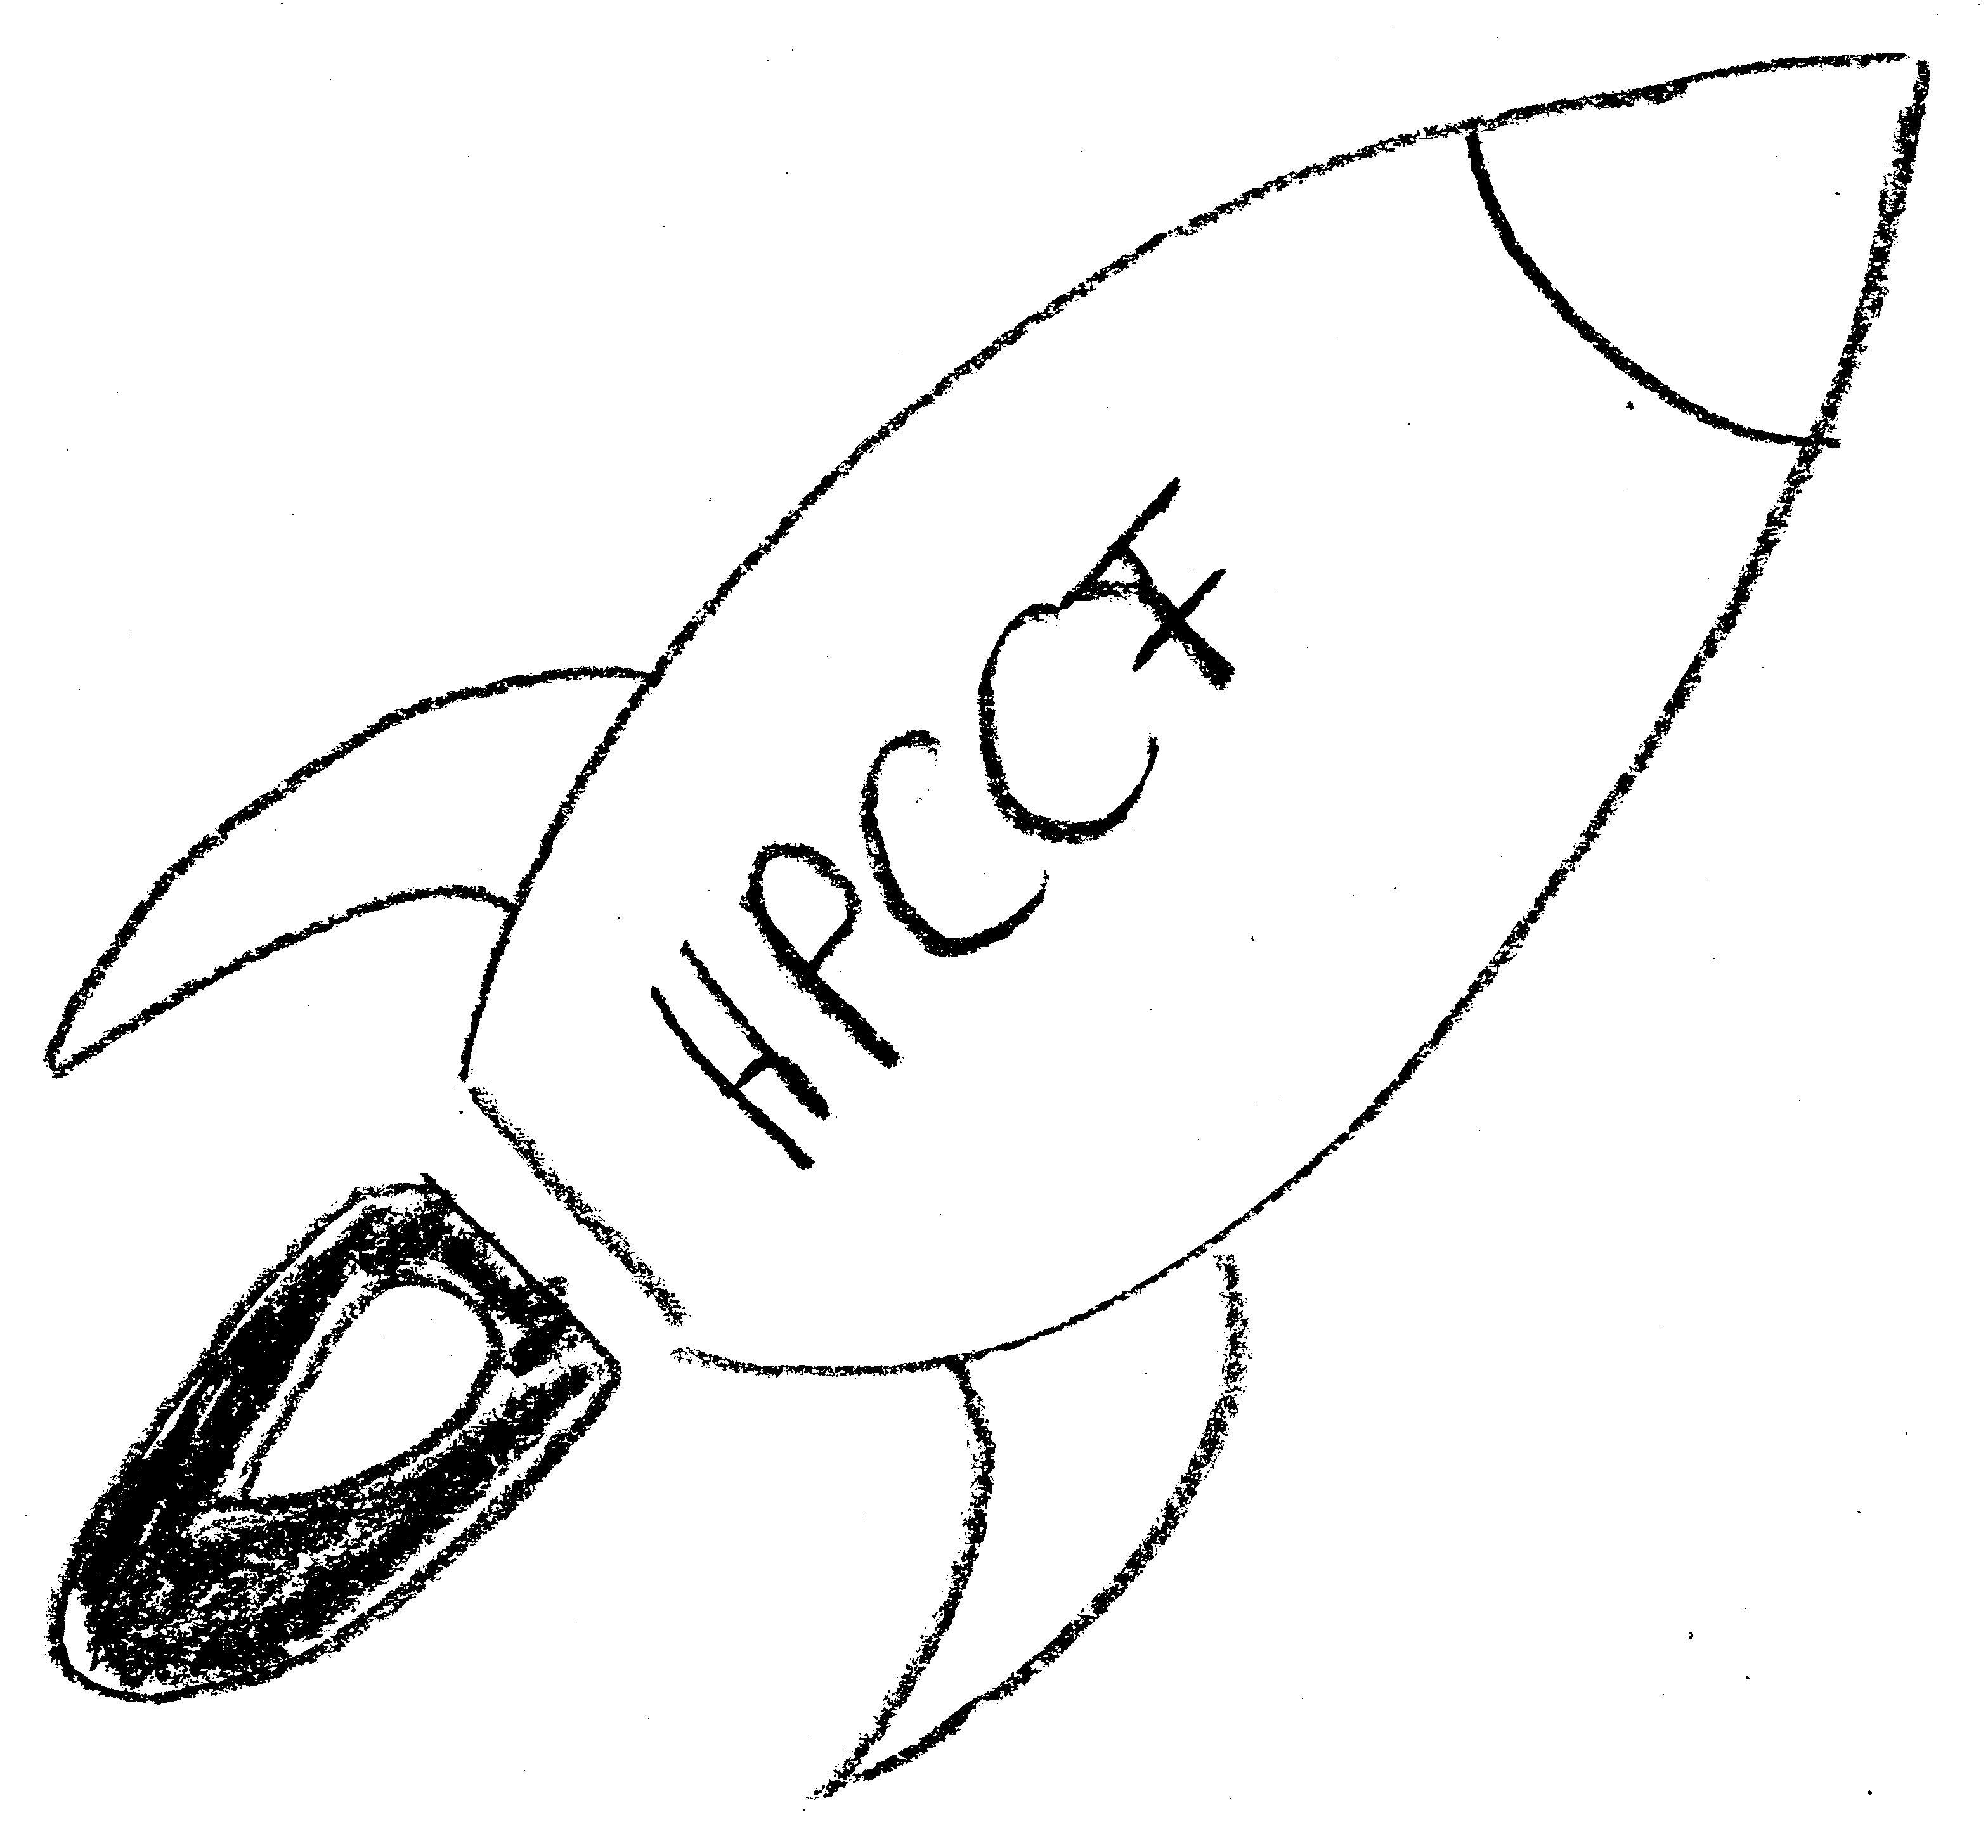
\includegraphics[width=0.6\textwidth]{images/hpccf_boost}
    \end{column}
  \end{columns}
\end{frame}

\begin{frame}
  \frametitle{Multiple Choice Questions}
  \begin{columns}
   \begin{column}{.5\textwidth}
      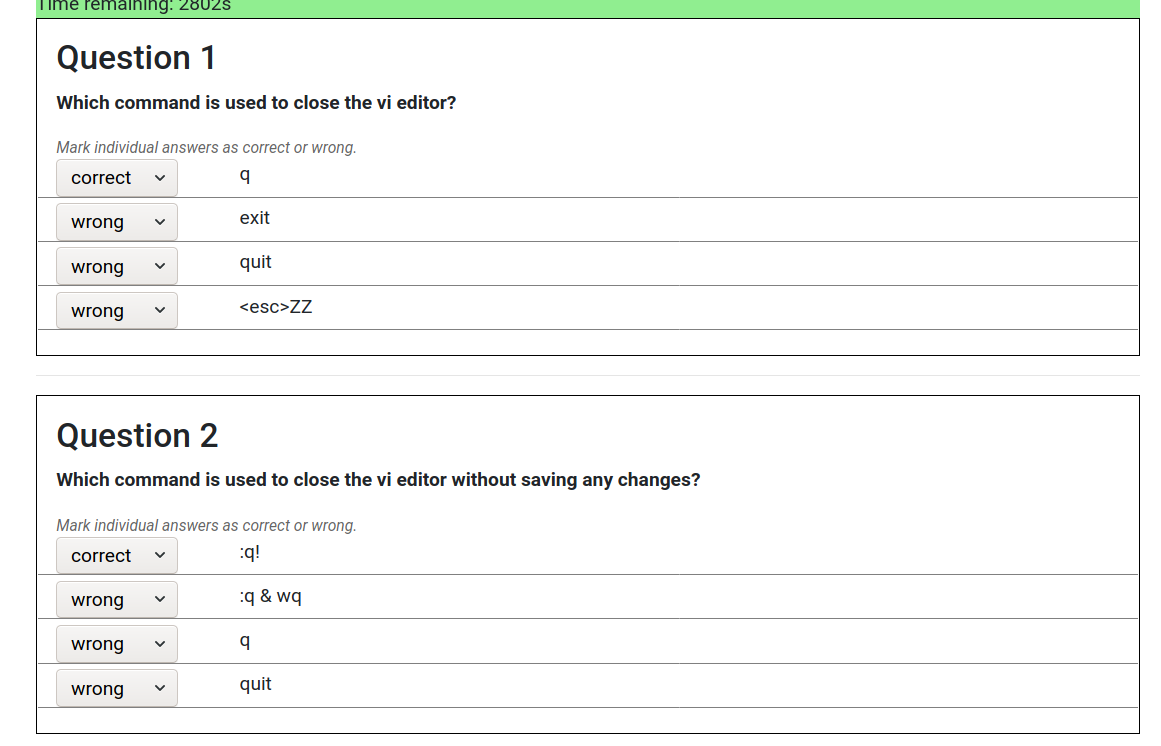
\includegraphics[width=0.9\textwidth]{images/questions_2}
   \end{column}
   \begin{column}{.5\textwidth}
       \centering
      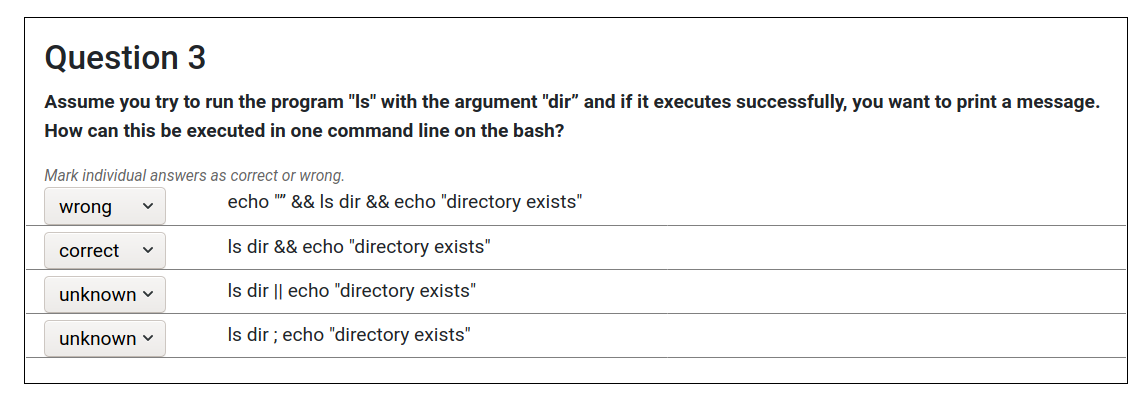
\includegraphics[width=0.9\textwidth]{images/question_1}
    \end{column}
  \end{columns}
\end{frame}

\begin{frame}
  \frametitle{Scenerio Based Questions}

\begin{tcolorbox}[colback=gray!5,colframe=green!40!black,title=Here:]
\footnotesize
In this task, you will need to run the program \texttt{terminator} and send a fixed sequence of signals to the program.
Note that this program is very sensitive to signals, very bad things may happen on the cluster if it is used incorrect. \textbf{Therefore, it is mandatory that you send the correct sequence of signals to the program and no other sequence.} 

We want to remind you that you can open multiple terminal sessions by opening the URL with the browser again.

Please send the following sequence of signals: 
\begin{enumerate}
  \item INT
  \item USR1
  \item 2
\end{enumerate}
\end{tcolorbox}

\end{frame}

\begin{frame}
  \frametitle{Scenerio Based Questions - Continued}
  \centering
  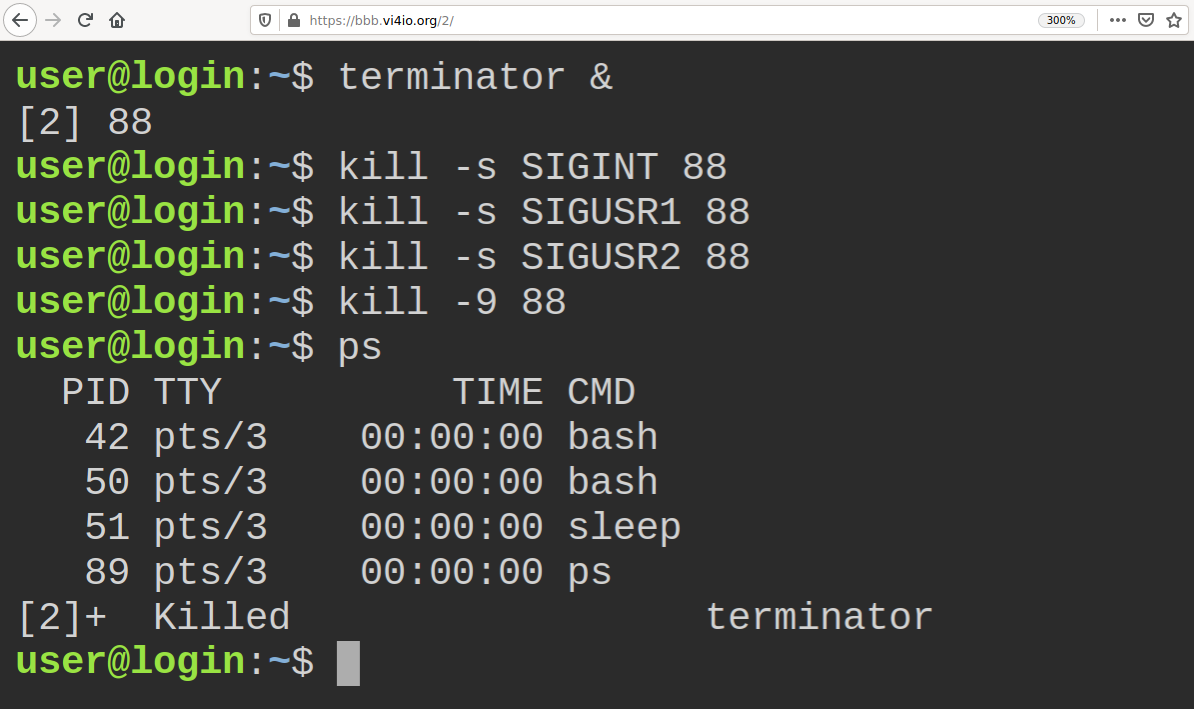
\includegraphics[width=0.65\textwidth]{szenario_3.png}

  Note: \texttt{SIGUSR2} != 2. Hence: Not full grade.
\end{frame}


% \begin{frame}
%   \frametitle{Improvements}
%   \begin{columns}[c, onlytextwidth]
%    \begin{column}{.4\textwidth}
%       \setlength{\partopsep}{0pt}
%       %\begin{minipage}{\textwidth}\vspace{0pt}
%        Bullet Point / Tick Boxes:\newline
%       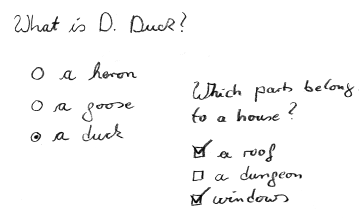
\includegraphics[width=0.9\textwidth]{mcq_ideal}
%       %\end{minipage}
% 
%       
%    \end{column}
%    \begin{column}{.55\textwidth}
%        \pause
%        \setlength{\partopsep}{0pt}
%       % \begin{minipage}{\textwidth}\vspace{0pt}
%         Syntax Highlighting:\newline
%       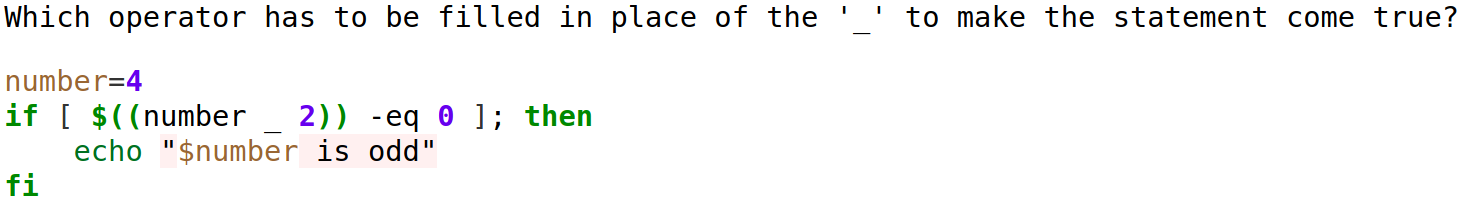
\includegraphics[width=0.9\textwidth]{syntax}\newline
%       \footnotesize{actual screenshot, not \LaTeX highlighting for the talk}
%        %\end{minipage}
% 
%       
%     \end{column}
%   \end{columns}
%   
% \end{frame}








%\section[Designing Questions]{design}

\begin{frame}
  \frametitle{Disclaimer}
  Some examples are inspired by Greg Wilsons book
 \begin{center}
  \sf{Teaching Tech Together} (CRC Press, 2020)
 \end{center}
 Some ideas are based on own experience, some on other sources.
\end{frame}

\subsection{Question Types}

\begin{frame}
  \frametitle{Purposes \ldots}
  Before diving into Question Design, note:
  \begin{itemize}
    \item a question can be asked with a certain aim
    \item different courses ask for different knowledge / skills
    \item $\curvearrowright$ questions need to be designed and choosen with care
  \end{itemize}
\end{frame}

% overview
% background selection

\subsection{Multiple Choice Questions}

\begin{frame}
 \frametitle{Multiple Choice -- When?}

 Multiple Choice Questions (MCQs) are popular when designing e-learning tests \ldots\vspace{-1em}
 \pause
 \newline
 \only<2->{\question{When are they most suitable?}}
 \pause
 Suppose you are teaching children and you give them this MCQ:
 \exercise[Testing Conceptions]{
  What is 37 + 15?
  \begin{enumerate}[a)]
   \item 52  {\color{pdarkgrey}correct}
   \item 42  {\color{pdarkgrey}child did not understand ``carrying''}
   \item 412 {\color{pdarkgrey}child treated every column seperately}
   \item 43  {\color{pdarkgrey}knows she has to carry 1, but to wrong column}
  \end{enumerate}
 }
\end{frame}


\begin{frame}
 \frametitle{Multiple Choice -- When? (continued)}
 
 The Young-Child question rephrased for newbies to the SLURM batch system:
 \vspace{-1em}
 \exercise[Testing Conceptions about SLURM]{
   Think of a cluster with 20 core nodes. If a job is submitted with the following parameterisation, how many nodes are reserved?\newline
   \texttt{\#SBATCH -n 20}\newline
   \texttt{\#SBATCH -c 2}
   \begin{enumerate}[a)]
    \item 2 {\color{pdarkgrey}correct}
    \item 4 {\color{pdarkgrey}user did correctly multiply, but is not aware of the 20 cores}
    \item 1 {\color{pdarkgrey}user did not multiply by \texttt{-c 2}}
    \item unkown without \texttt{N}-flag {\color{pdarkgrey}user did not understand the concept}
   \end{enumerate}
  }
\end{frame}

\begin{frame}
  \frametitle{What is in the Arsenal?}
  \begin{columns}
   \begin{column}{.5\textwidth}
    MCQs aren't everything:
     \begin{enumerate}
      \item Freetext (if short and explicit)
      \item Filling in blanks (for code; to be implemented)
      \item Parson Problem (can by done as MCQ; in a minute)
      \item Tracing (can by done as MCQ; in a minute)
     \end{enumerate}
   \end{column}
   \begin{column}{.5\textwidth}
       \centering
      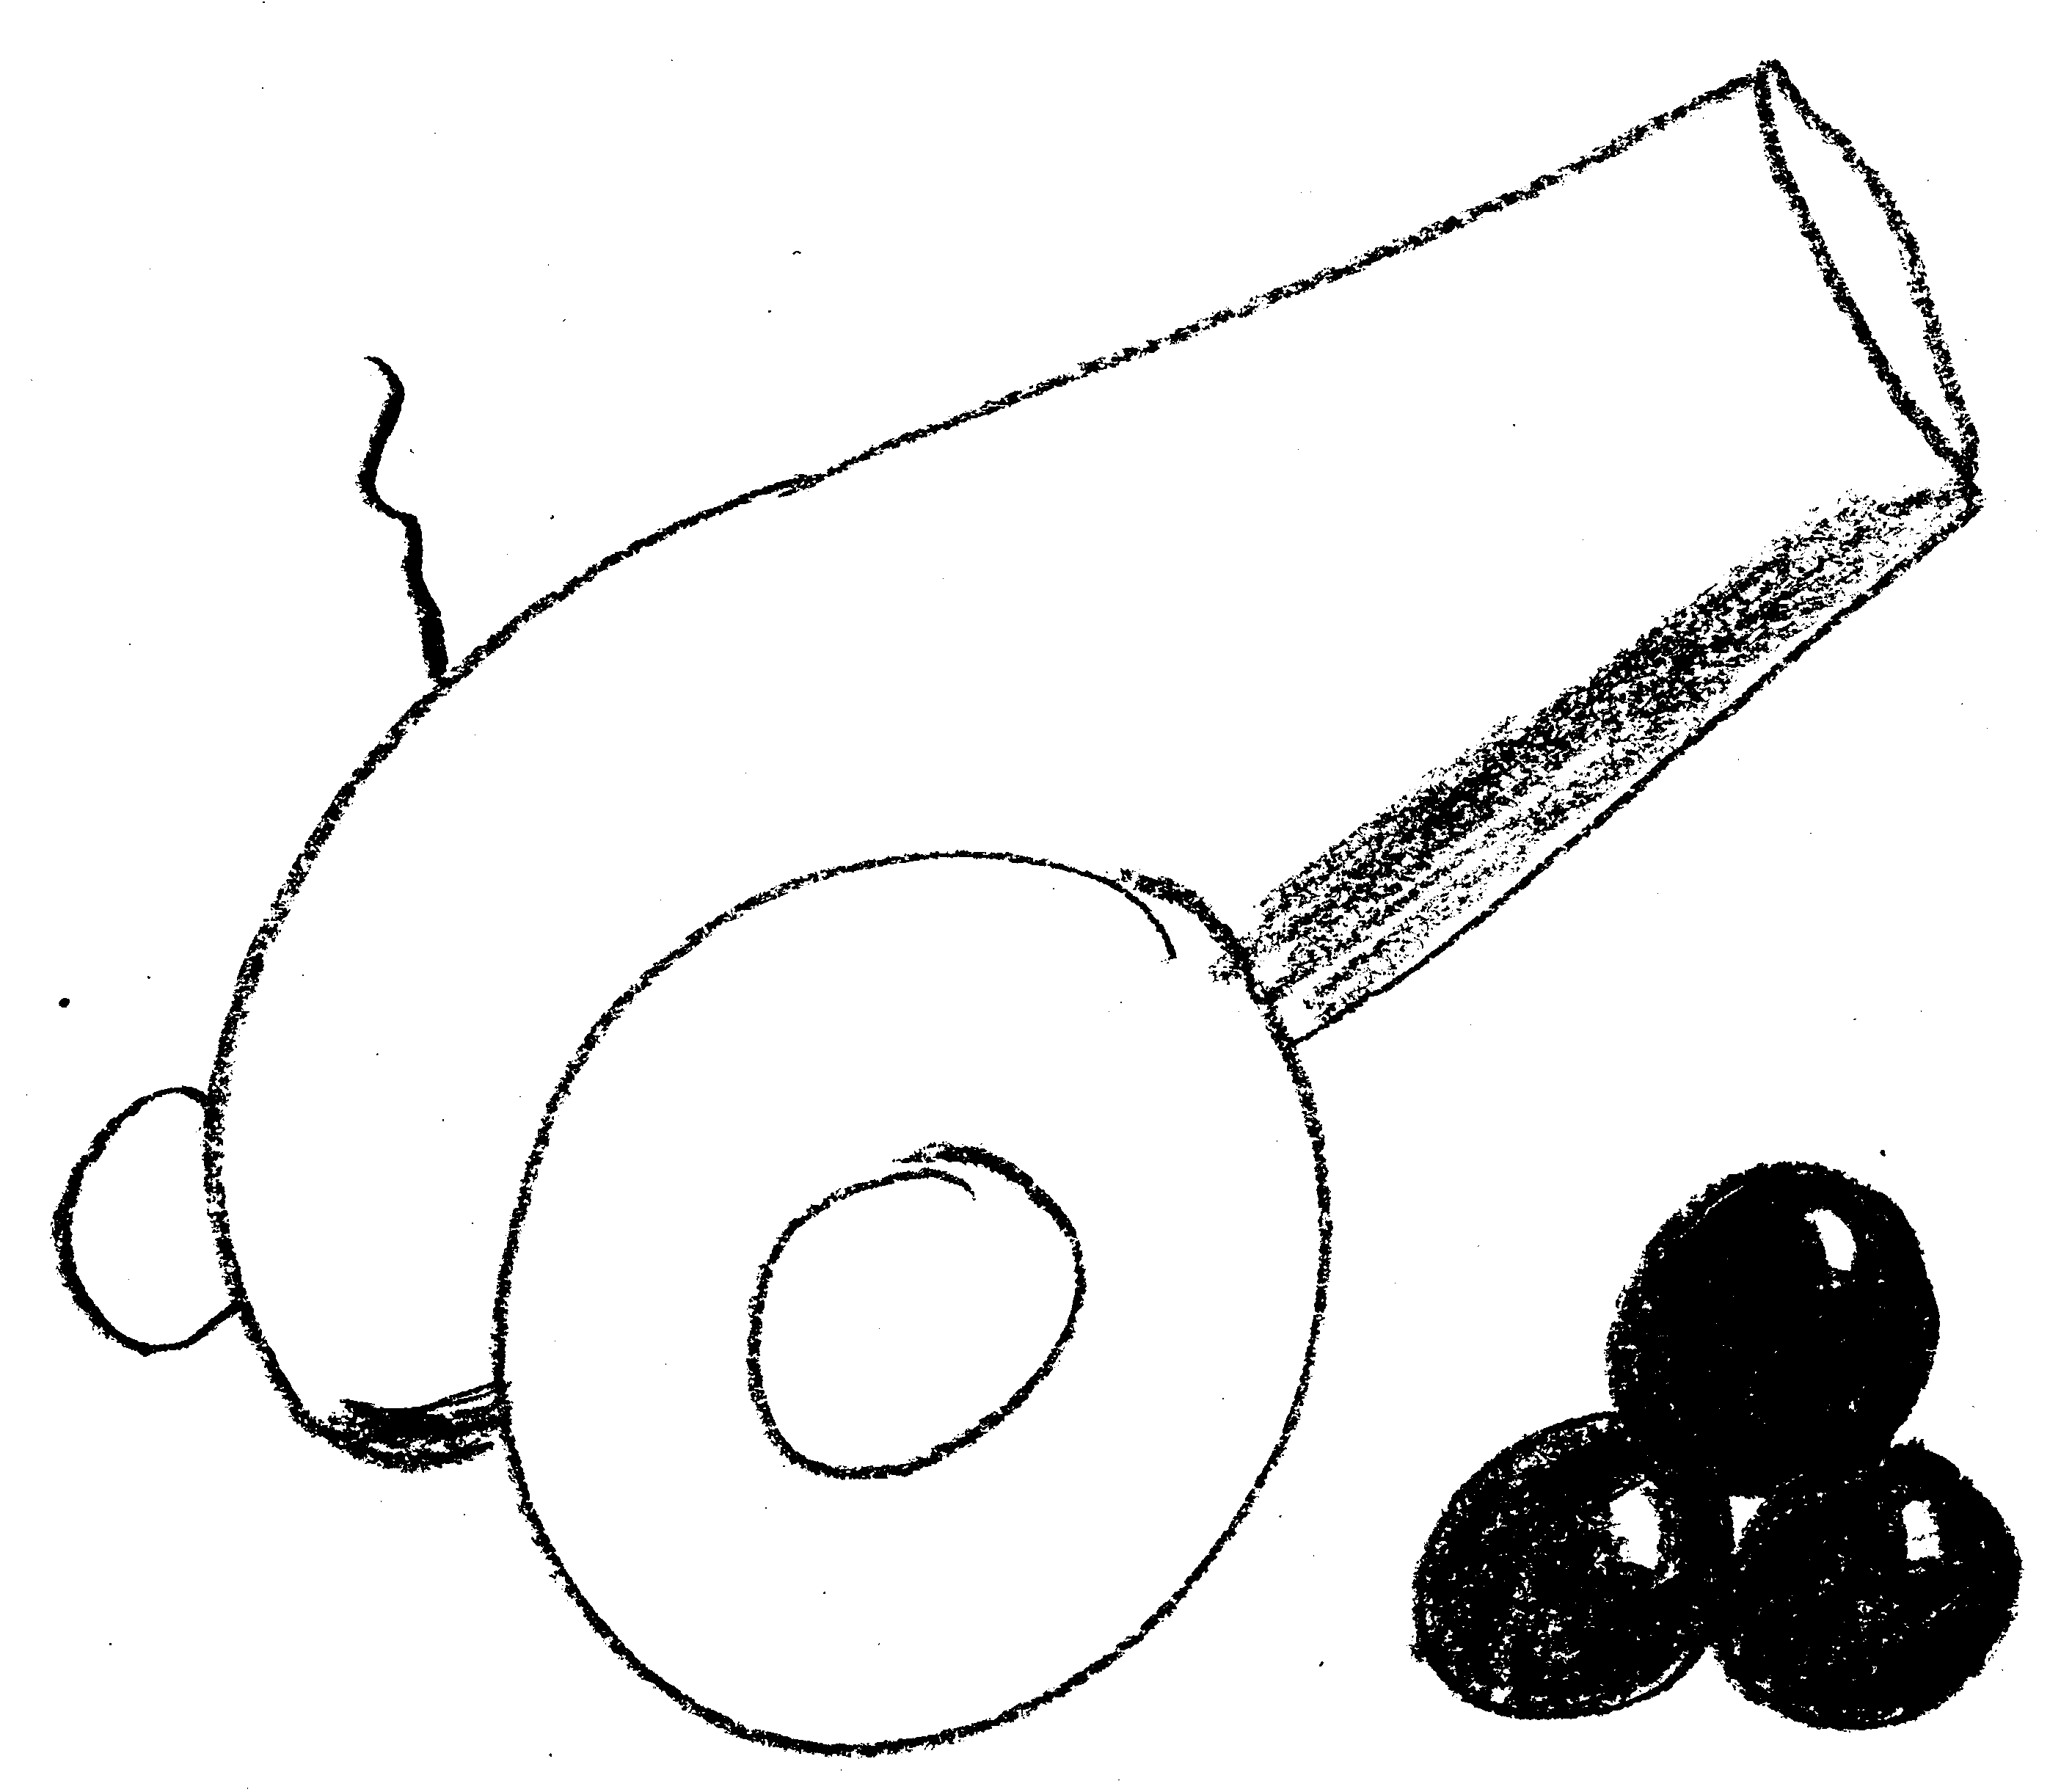
\includegraphics[width=0.6\textwidth]{images/arsenal}
    \end{column}
  \end{columns}
\end{frame}

\begin{frame}
  \frametitle{Freetext}
  Freetext question need to be \emph{very} much restricted to simple words or characters. For example:
  \exercise[Changing Permissions]{
           If a script file 'foo.sh' has the permissions '-rw-r--r--', 
           how do make it executable for your group for sharing the script?
           }
  Here, only two possible answers are allowed, in octal or explicit mode.
  \pause
  \hint[Most Suitable]{This kind is of question is most suitable to test actual knowledge. As we can expect only few students to memorize all nifty details, it primarly tests for gained experience and is to be used with great care (not to frequent).}
\end{frame}

\begin{frame}
  \frametitle{Fill in Blanks}
  Filling Blanks is a (technical) variation on Freetext. It is more specific and the \emph{blank screen of horror} problem, whilst testing vocabulary. An example:
  \exercise[Bash Operators]{
            Which operator has to be filled in the place of '\_' to print the statement in line 3?\newline
            {\small \bf 1:} \texttt{number=4}\newline
            {\small \bf 2:} \texttt{if [ \$((number {\color{red}\bf\_} 2 )) -eq 0 ]; then}\newline
            {\small \bf 3:} \texttt{~~~~echo "\$number is even"}\newline
            {\small \bf 4:} \texttt{fi}
            }
  \hint{The answer is a single character.}
\end{frame}

\begin{frame}
  \frametitle{Parsons Problems}
  Parsons Problems, too, avoid the \emph{blank screen of horror} problem and also the vocabulary testing. Instead they allow the examinee to concentrate on the control flow. 
  \vspace{-.5em}
  \begin{columns}
    \begin{column}{.7\textwidth}
      \exercise[Bash Loop \& Math]{
                Rearrange these lines to sum the values.\newline
                {\small \bf 1:} \texttt{done}\newline
                {\small \bf 2:} \texttt{values=(1 2 3 4)}\newline
                {\small \bf 3:} \texttt{for v in \${values[@]}; do}\newline
                {\small \bf 4:} \texttt{total=\$((total + v))}\newline
                }
    \end{column}
    \begin{column}{.3\textwidth}
      Real tasks can be longer and intricated - allowing test of control flow understanding.
    \end{column}
  \end{columns}
  \vspace{-.5em}
  \hint[Note]{The answer can be a free text, e.\,g.: ``2 3 4 1'', which is easy to parse and check.}
\end{frame}

\begin{frame}[t]
  \frametitle{What else?}
  We could go on \ldots
  \vspace{1em}
  \begin{columns}
    \begin{column}{.7\textwidth}
      \centering
      \begin{tabular}{p{.25\textwidth}p{.55\textwidth}}
         Exercise Type & Technical Implementation\\\hline
         Tracing Code Execution & \only<2->{Freetext or MCQ}\\
         Labelling Diagrams & \only<3->{MCQ}\\
         Fixing Code & \only<4->{Freetext}\\
         etc & \only<5->{Variety of types with minimal technical effort.}
      \end{tabular}
    \end{column}
    \begin{column}{.3\textwidth}
      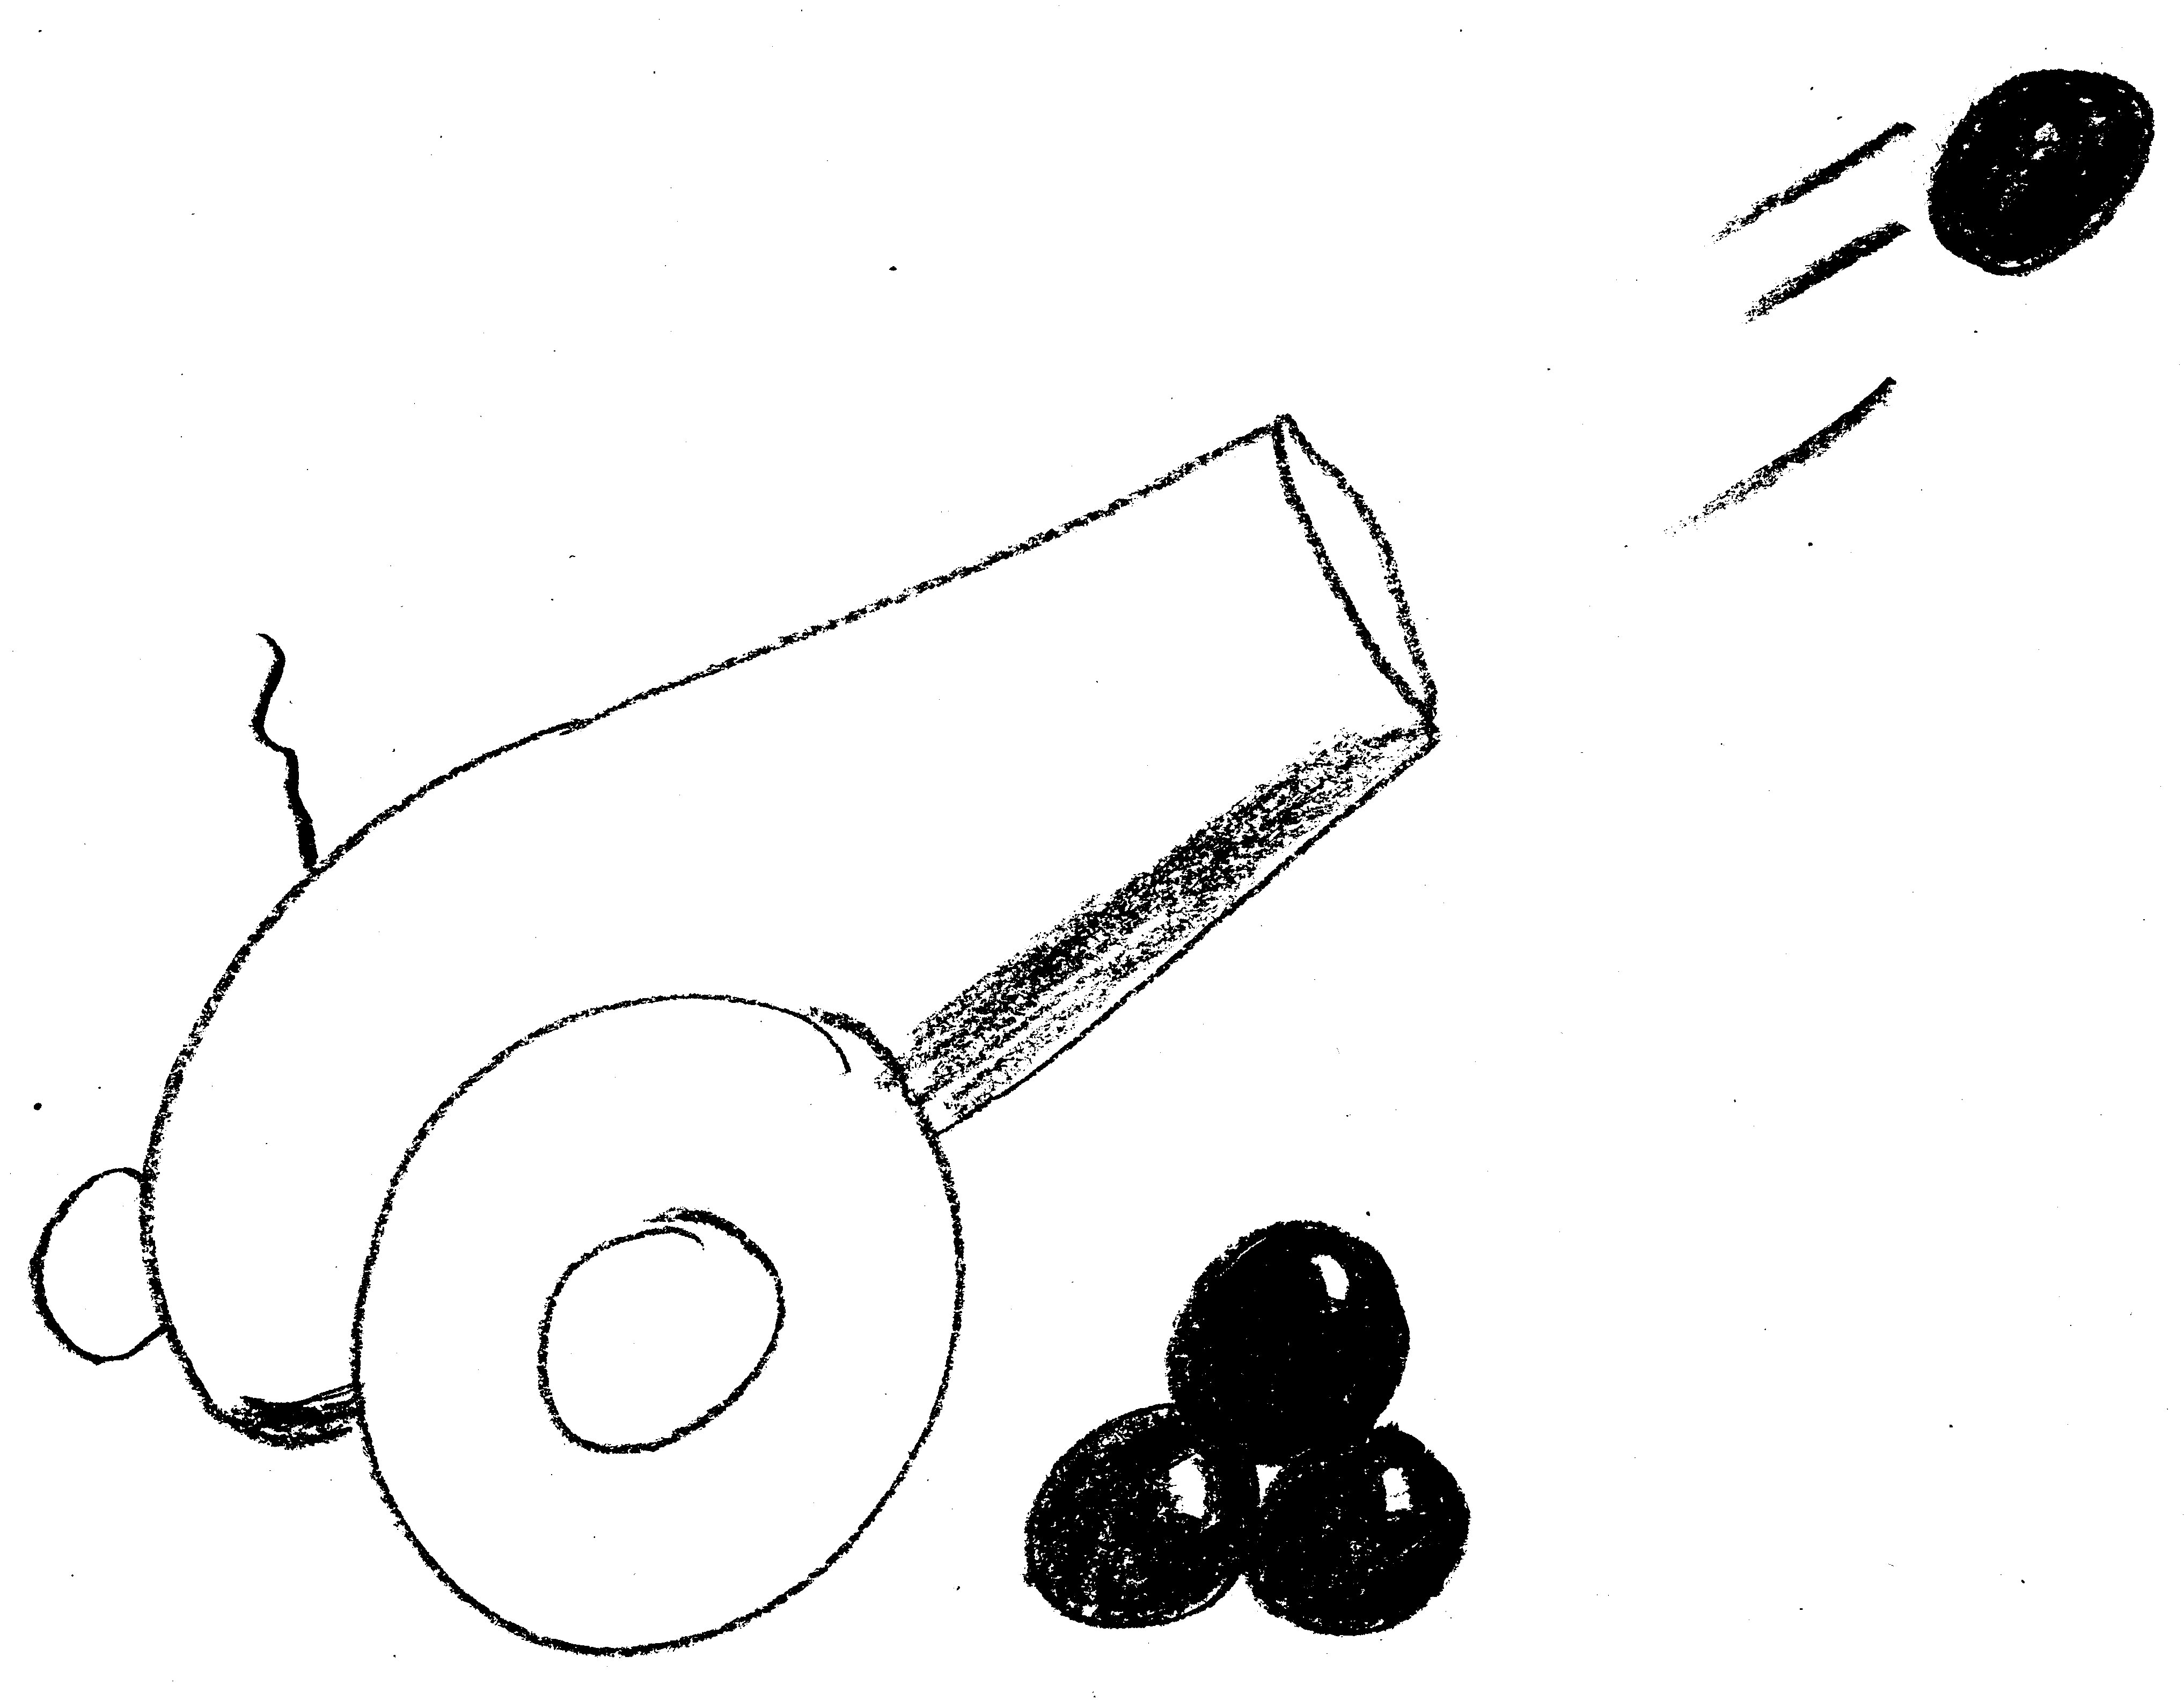
\includegraphics[width=0.6\textwidth]{images/arsenal2}
    \end{column}
   \end{columns}
\end{frame}



%\section[Contributing to the Question Pool]{Contributing}

\begin{frame}
  \frametitle{Contributions via the HPCCF-Wiki}
  \centering
  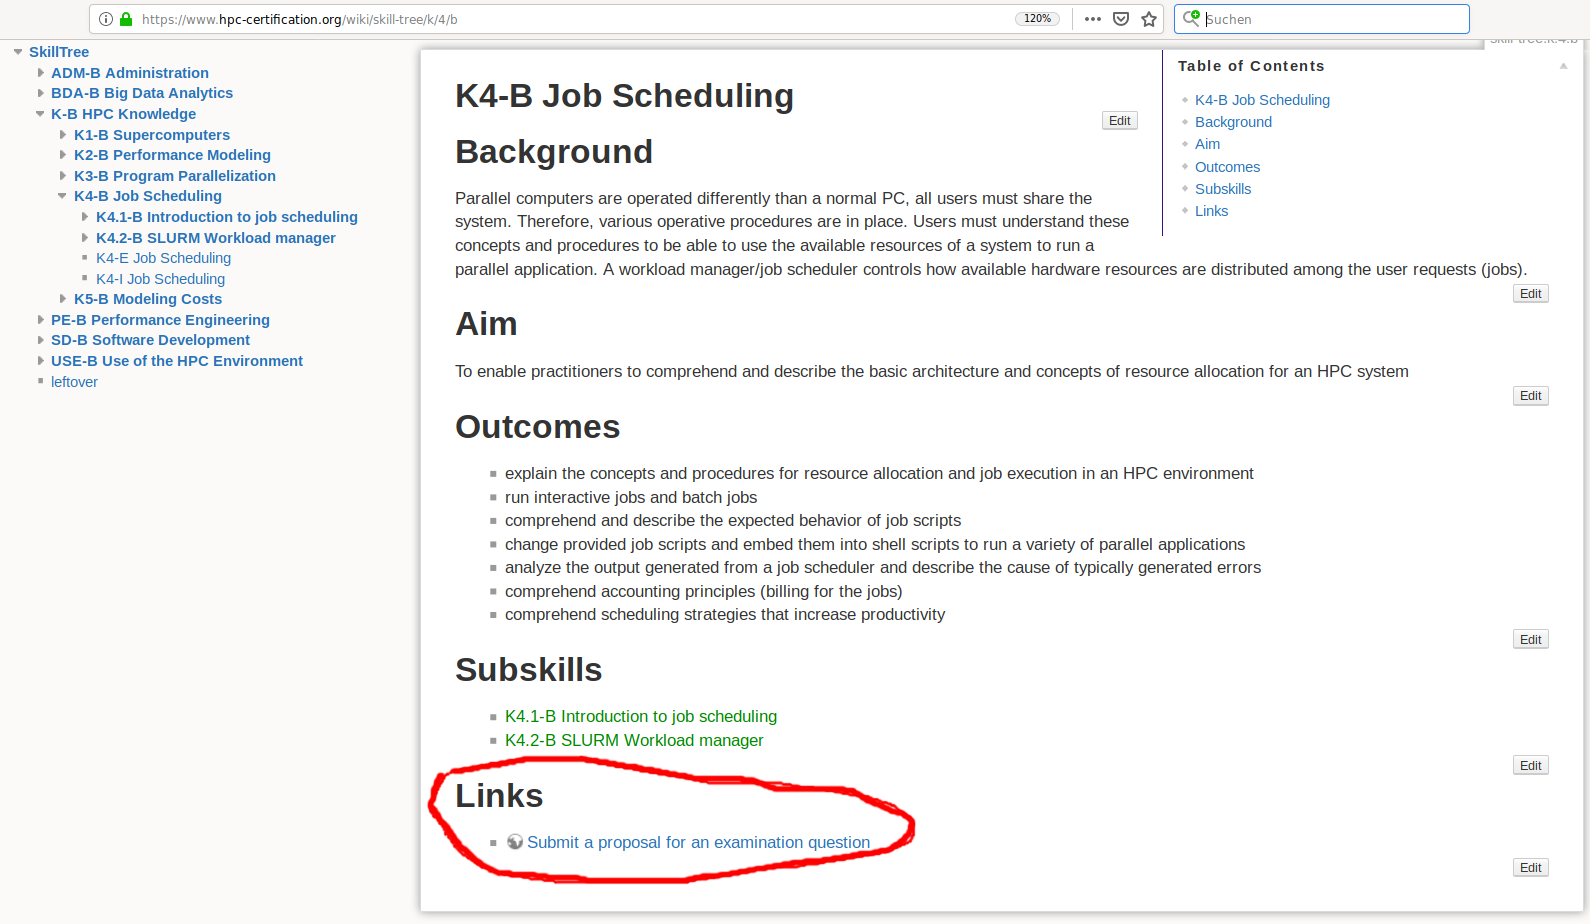
\includegraphics[width=0.8\textwidth]{images/contribution}
\end{frame}


\begin{frame}
  \frametitle{Contributions via the HPCCF-Wiki II}
  Each \lhref{https://www.hpc-certification.org/wiki}{HPCCF wiki} page contains a link. It leads to a little form asking for:
  \begin{itemize}
   \item contact mail
   \item to select a learning objective from a pre-formatted list
   \item to supply the question you thought of
   \item and (in case of a multiple choice question) the possible answers.
  \end{itemize}
  \pause
  \task[Evaluation Process]{Now, HPCCF-member evaluate the submitted question. If approved, it will be formatted and merged into the pool of questions for the choosen topic / skillset.}
\end{frame}



\begin{frame}
 \centering
 \begin{columns}
   \begin{column}{0.8\textwidth}
     \centering
     \Large
     Thank You for Your Attention!
   \end{column}
   \begin{column}{0.2\textwidth}
     
      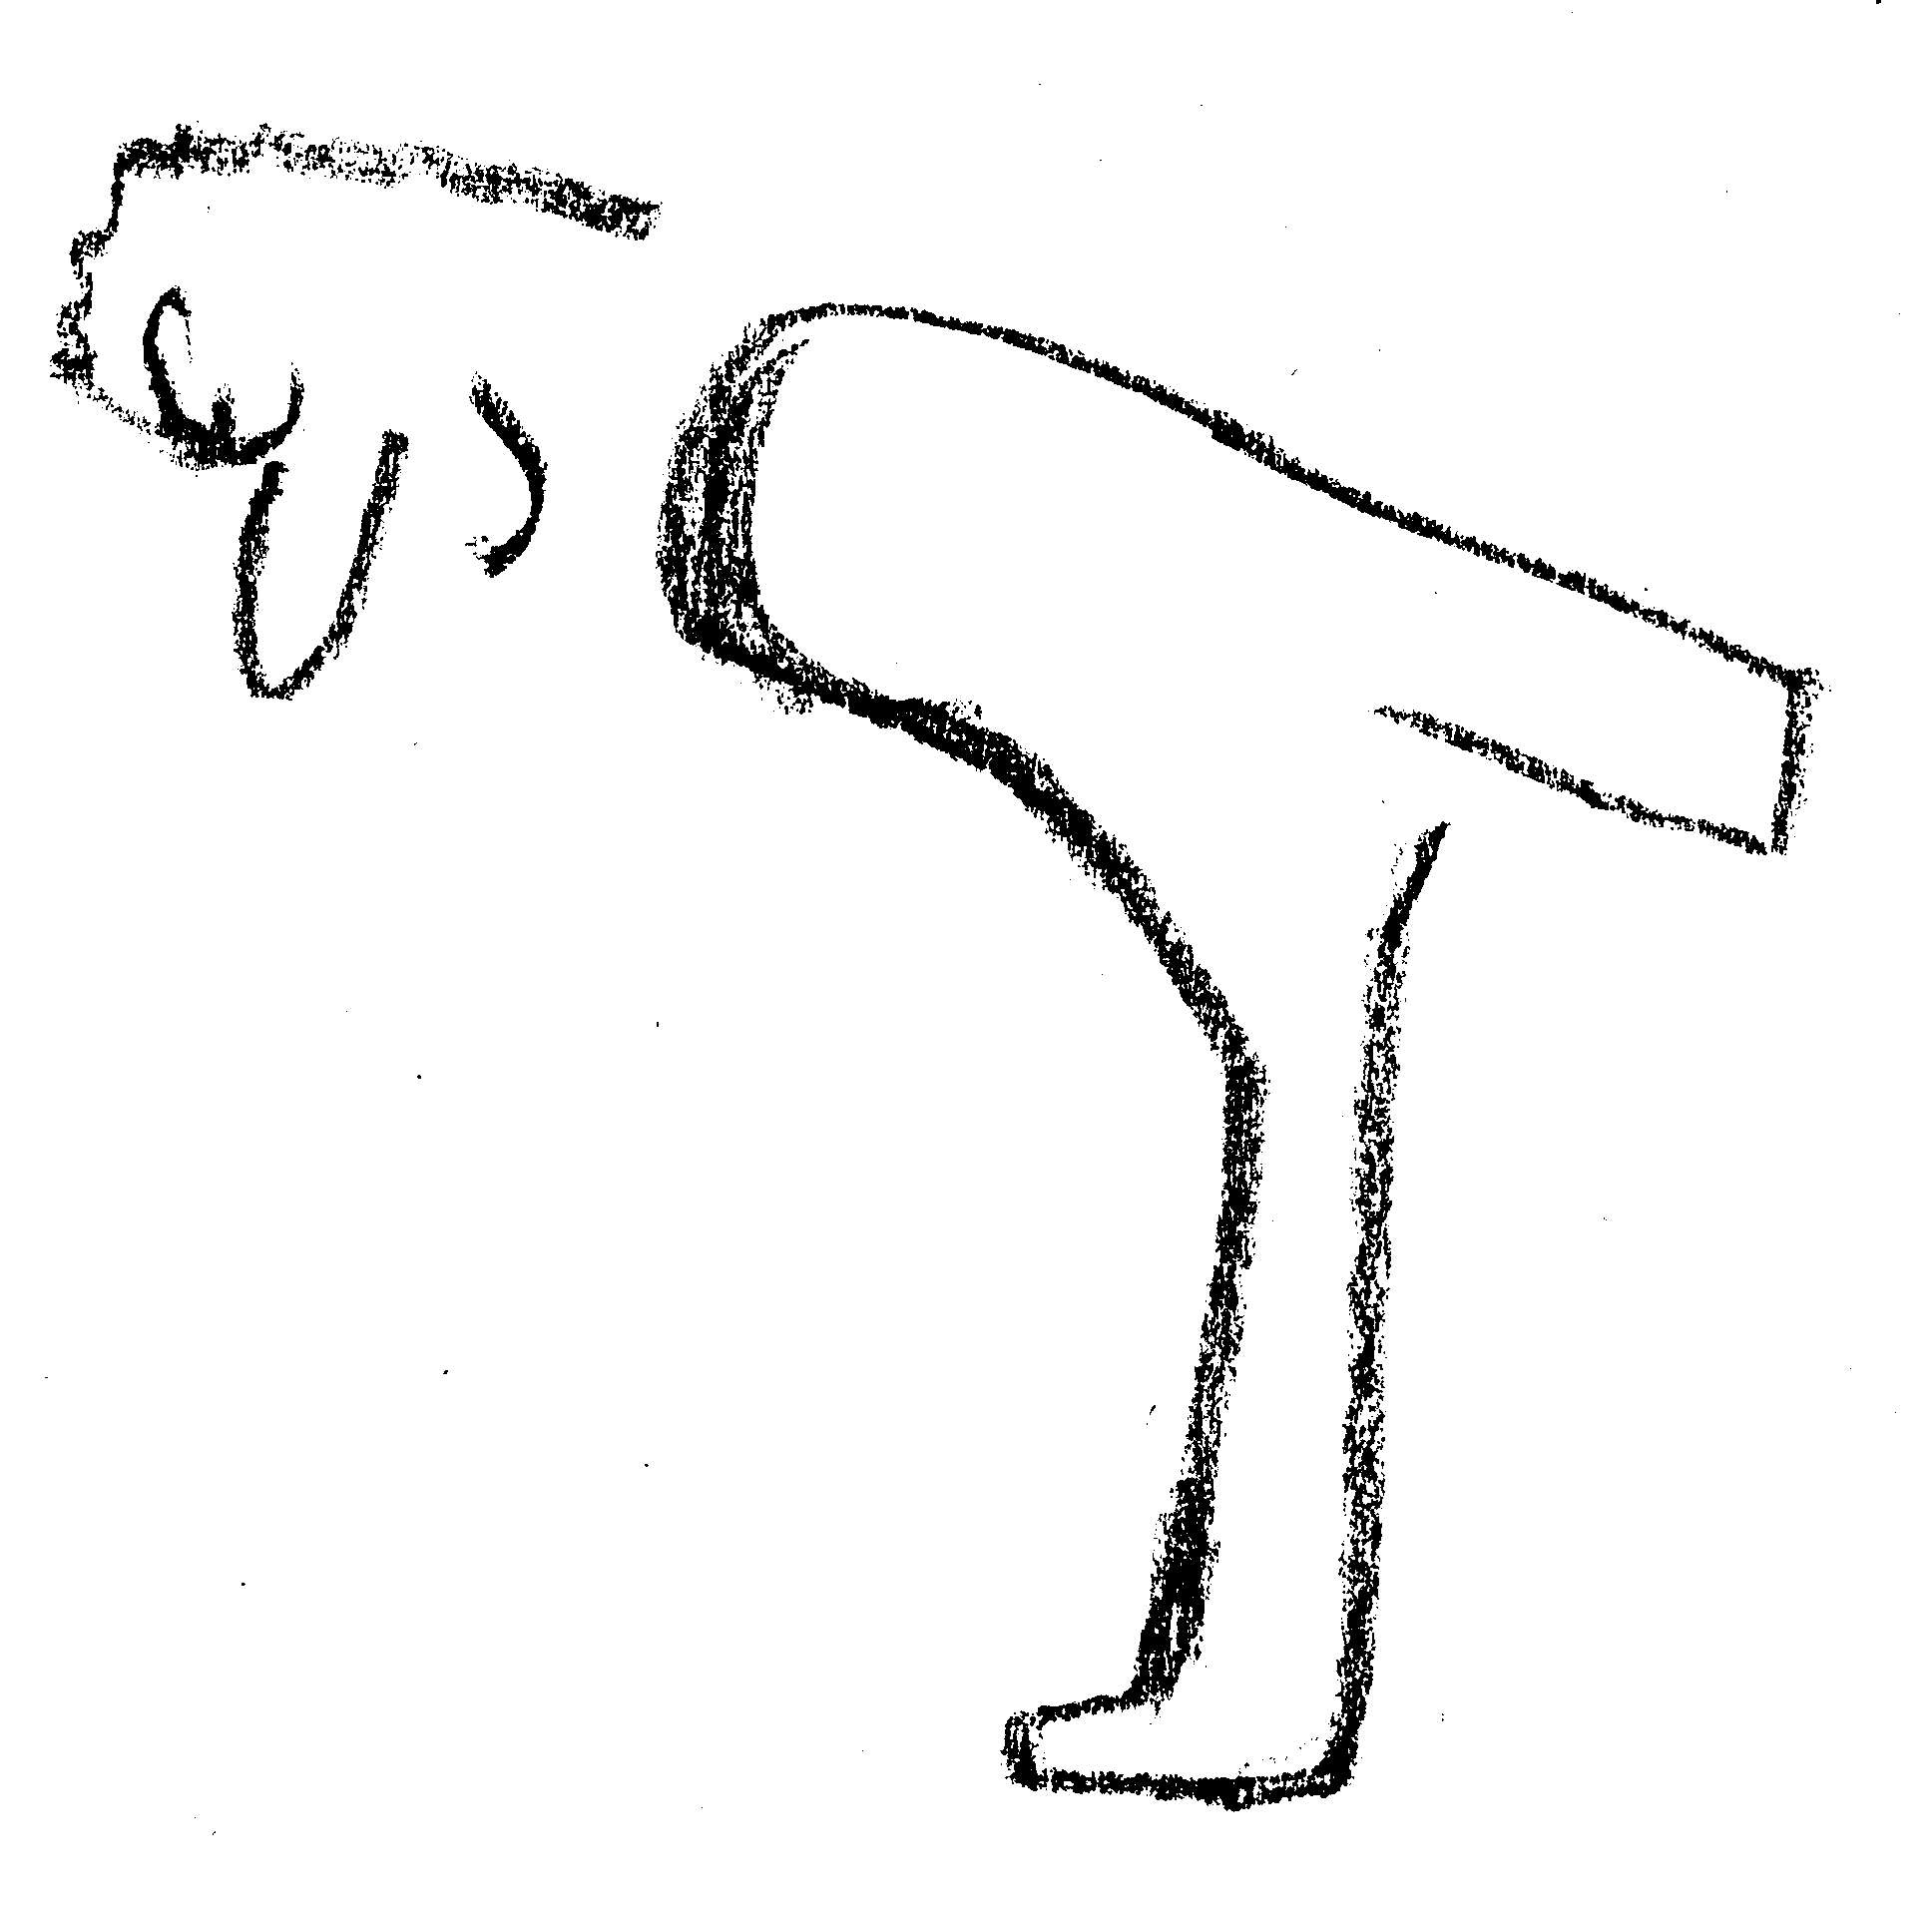
\includegraphics[width=.6\textwidth]{images/end}
   \end{column}
 \end{columns}
\end{frame}


\end{document}

